\chapter{Resultados}
\label{capitulo 3}

En este capítulo se muestran los resultados obtenidos al entrenar los modelos previamente descritos, 
el objetivo es predecir los caudales de descarga naturales en cada una de las sub-cuencas que conforman CHRC para  un evento de 
precipitación dado. 
La performance predictiva de los modelos es evaluada en el conjunto de test, 
en la tabla \ref{hyperres} se muestran los hyper-parámetros utilizados para cada modelo obtenidos
tras realizar la exploración descrita en \ref{cal}.


\begin{table}[]
  \begin{center} 
  \begin{tabular}{|l|l|l|l|l|l|}
    \hline
   Modelo&optimizador &Neuronas & Activación & alpha & reg \\
   \hline
   Denso & rmsprop& 200& relu & 0.0002 &l2, 0.0001  \\
   LSTM1 PCA & rmsprop  &200 & linear &  0.0002  & l2, 0.0001 \\
   LSTM1 loc & adam & 200 & relu & 0.0001 &  l1, 0.0001  \\
   LSTM2 & adam & 200 & relu &  0.001 & l2, 0.0000001 \\
  
   \hline

  \end{tabular}
  \caption{ Hyper parámetros utilizados en los diferentes modelos.}
  \label{hyperres}
\end{center}
  \end{table}

\section{Validación de los modelos}


 \begin{figure}[h!]
   \begin{center}
     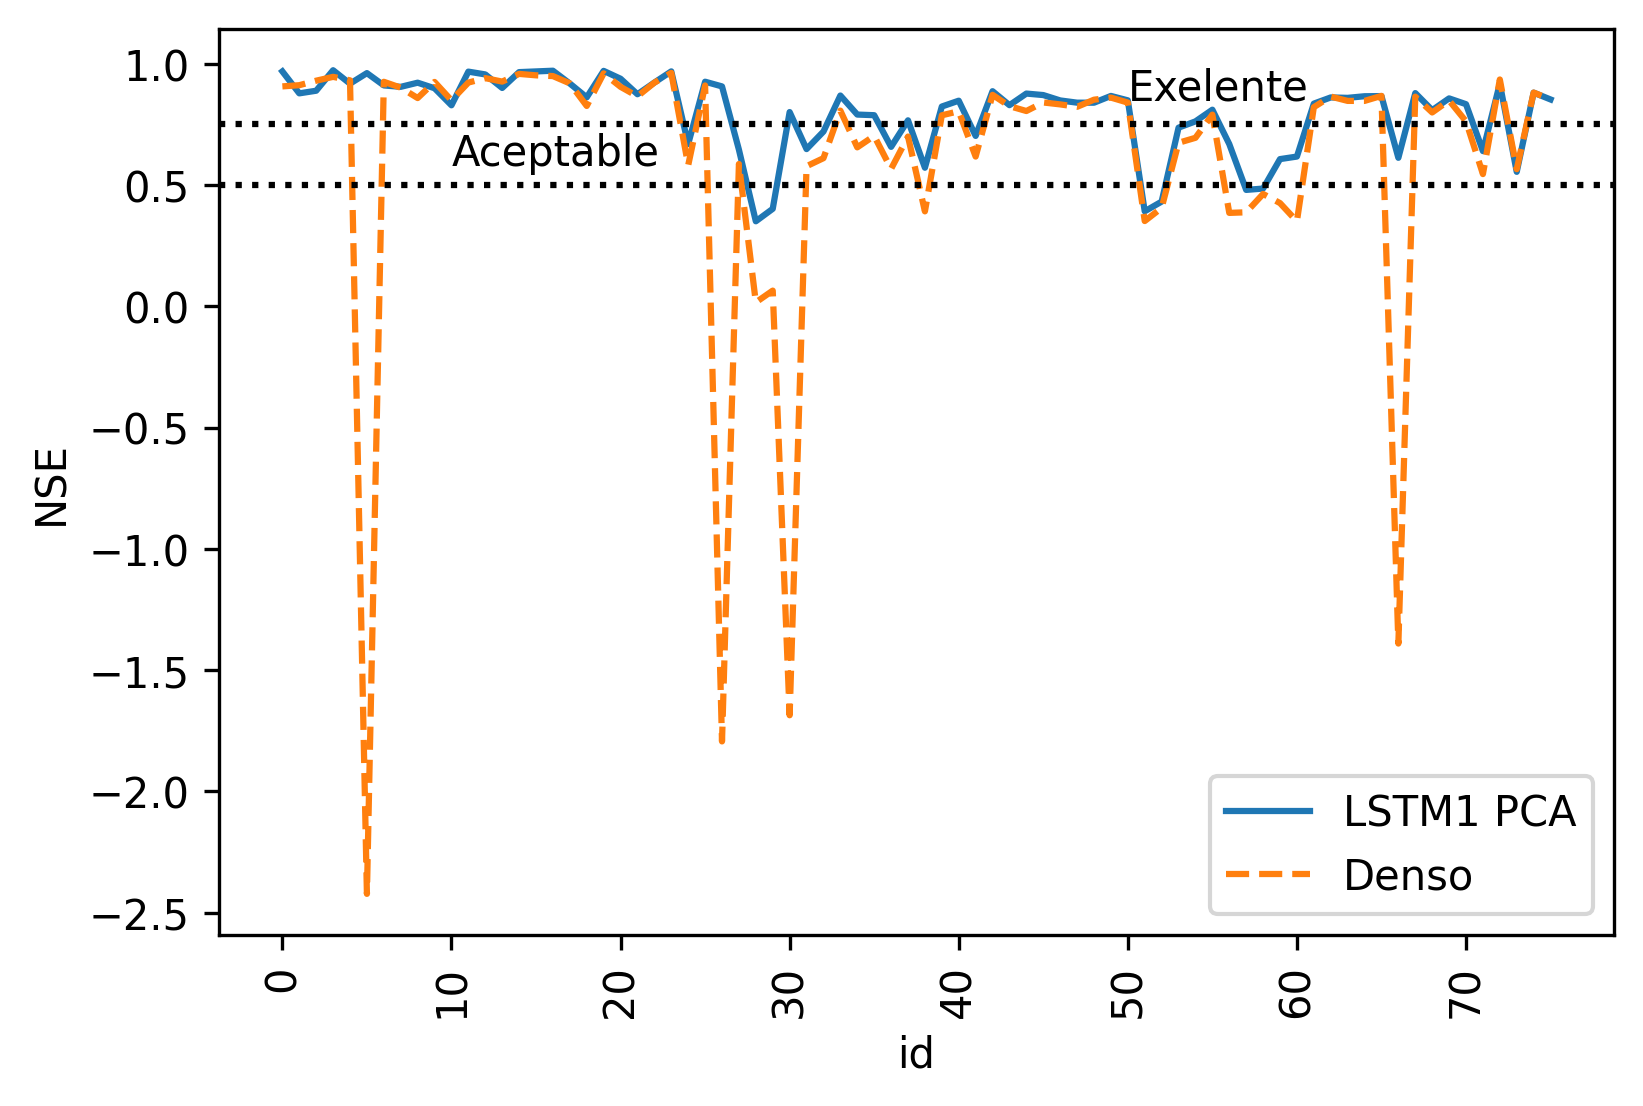
\includegraphics[height=3.in]{Figures/NSE/NSEs_LSTM1s_PCA.png}
     \caption{ Valores obtenidos para el coeficiente NSE a lo largo de toda la cuenca con los modelos denso
     y LSTM1 entrenado con PCAs.}
     \label{NSE1}
   \end{center}
 \end{figure}


Como se ha mencionado en la sección \ref{sectNSE}, se ha utilizado el coeficiente de Nash-Sutcliffe para
validar los modelos y hacer un análisis un poco más profundo sobre cómo es su performance en los diferentes puntos
de la cuenca. En la figura \ref{NSE1} se muestran los valores obtenidos 
de NSE para todas las sub-cuencas de Chambo considerando el modelo denso y el modelo LSTM1 entrenado de manera global 
en el espacio de las componentes principales. Las líneas horizontales muestran los umbrales correspondientes a 
ajustes excelentes y aceptables. 

El modelo LSTM1 posee una mejor performance general a lo largo de toda la cuenca, 
en este caso se  puede considerar que el ajuste para el 68$\%$ de las sub-cuencas es excelente, 
mientras que el 11$\%$ de los ajustes son buenos y el 16$\%$  aceptables. 
Por otro lado, si bien la performance general del modelo denso es buena (el 68$\%$ es mayor a $0.65$), 
el porcentaje de fallos asciende al 13$\%$. Se puede observar que en las subcuencas con ids 5, 26, 31 y 66 el coeficiente NSE adquiere 
valores negativos, mientras que el modelo LSTM1 realiza muy buenos ajustes.
La mejor performance del modelo LSTM1 se debe a que las celdas de memoria permiten una interpretación a lo largo del eje del tiempo de 
los diferentes procesos que ocurren en cada una de las cuencas, lo que permite captar más información sobre la relación entre
eventos de precipitación y descarga. 


\begin{figure}[h!]
  \begin{center}
    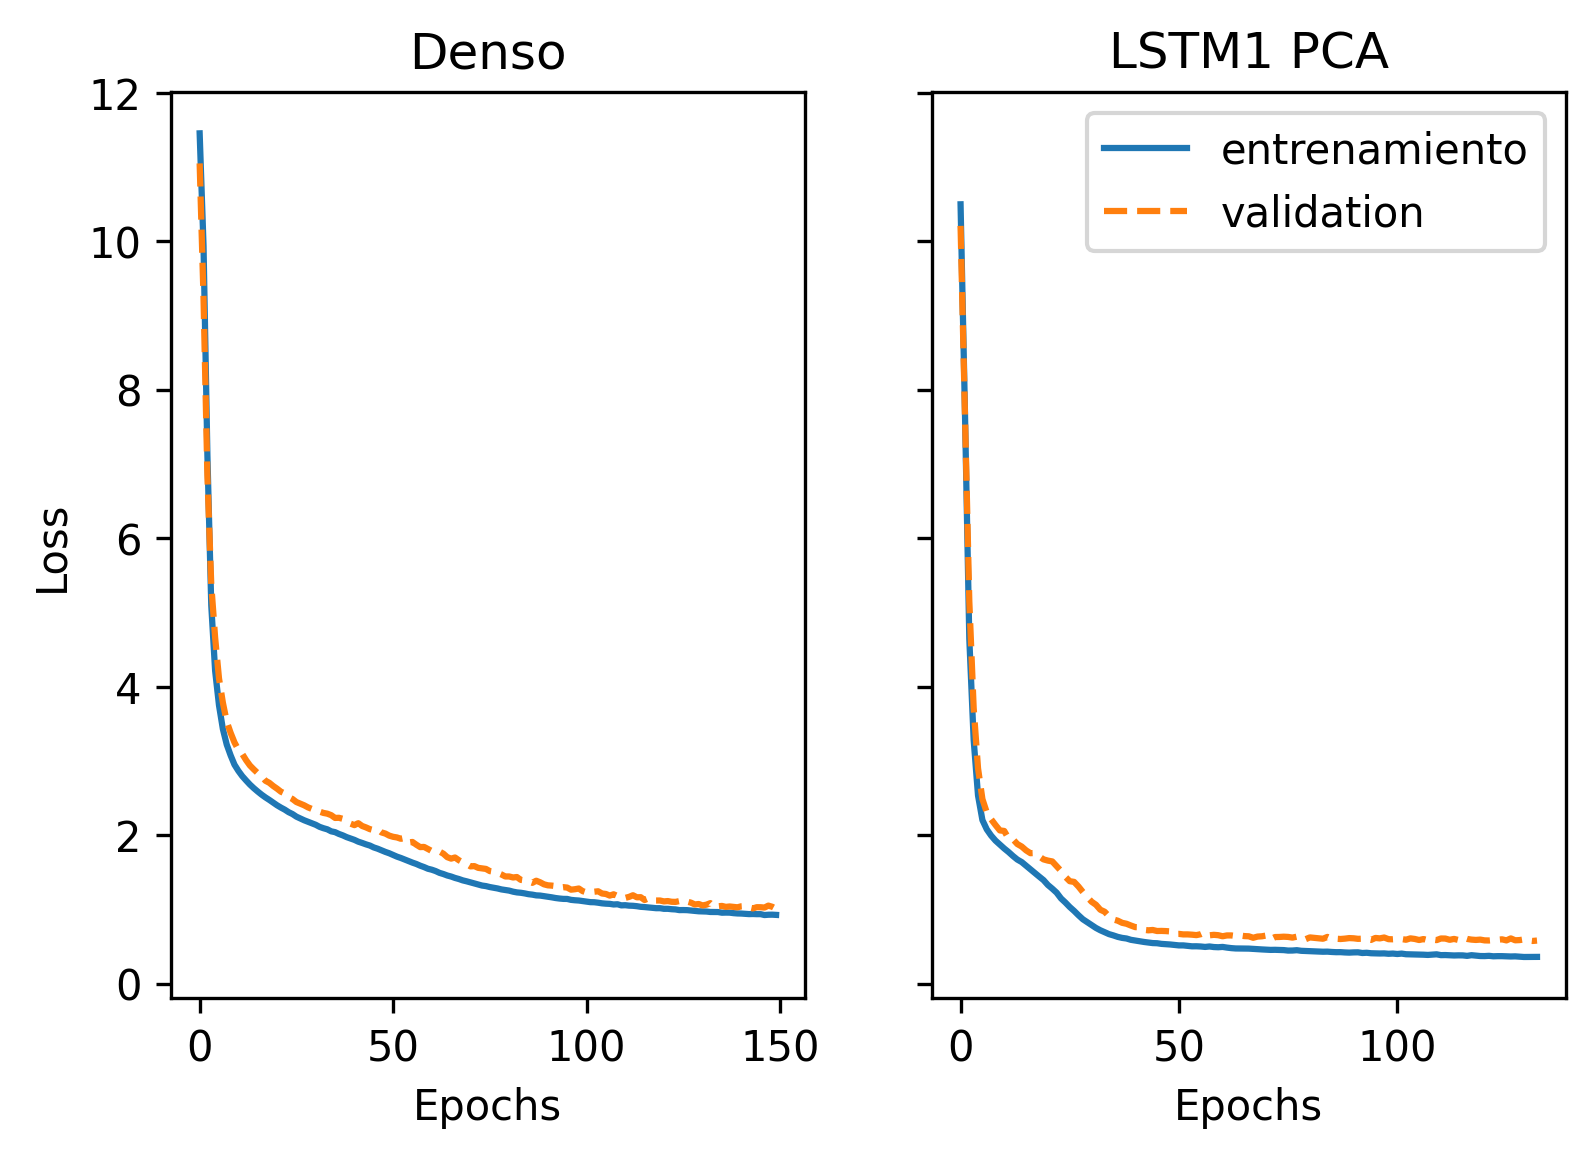
\includegraphics[height=3.in]{Figures/loss/comp_loss.png}
    \caption{ Evolución de la función de loss en los conjuntos de entrenamiento y validación para los modelos denso y
    LSTM1 con PCAs.}
    \label{losscomp}
  \end{center}
\end{figure}

En la figura \ref{losscomp} se muestran los valores de la función de loss obtenidos en cada época o iteración durante el entrenamiento
de los modelos denso y LSTM1 PCA.  Durante el entrenamiento se ha dividido el conjunto de datos de manera que el 
85$\%$ de los mismos han sido utilizados para entrenar el modelo y el 15$\%$ restante para validarlo y así evitar el sobre ajuste
monitorizando la evolución del loss. Además se ha implementado el callback "\textit{early sttoping}" que 
interrumpe la ejecución cuando el loss en el conjunto de validación comienza a aumentar.

Si se comparan ambos modelos, podemos observar que
en el modelo LSTM1 PCA aprende más rápido ya que en aproximadamente 50 épocas el valor de loss alcanza su valor de equilibrio, 
en el caso del modelo denso, esto ocurre luego de 150 épocas. Por otro lado, y en concordancia con los resultados
arrojados por el coeficiente NSE, el valor final del loss en el modelo LSTM1 PCA (entrenamiento: 0.3587 , validación: 0.5787)
es menor que en el modelo denso (entrenamiento: 0.9245 validación: 1.0060) los que indica un mejor ajuste global. 


  \begin{figure}[h!]
    \begin{center}
      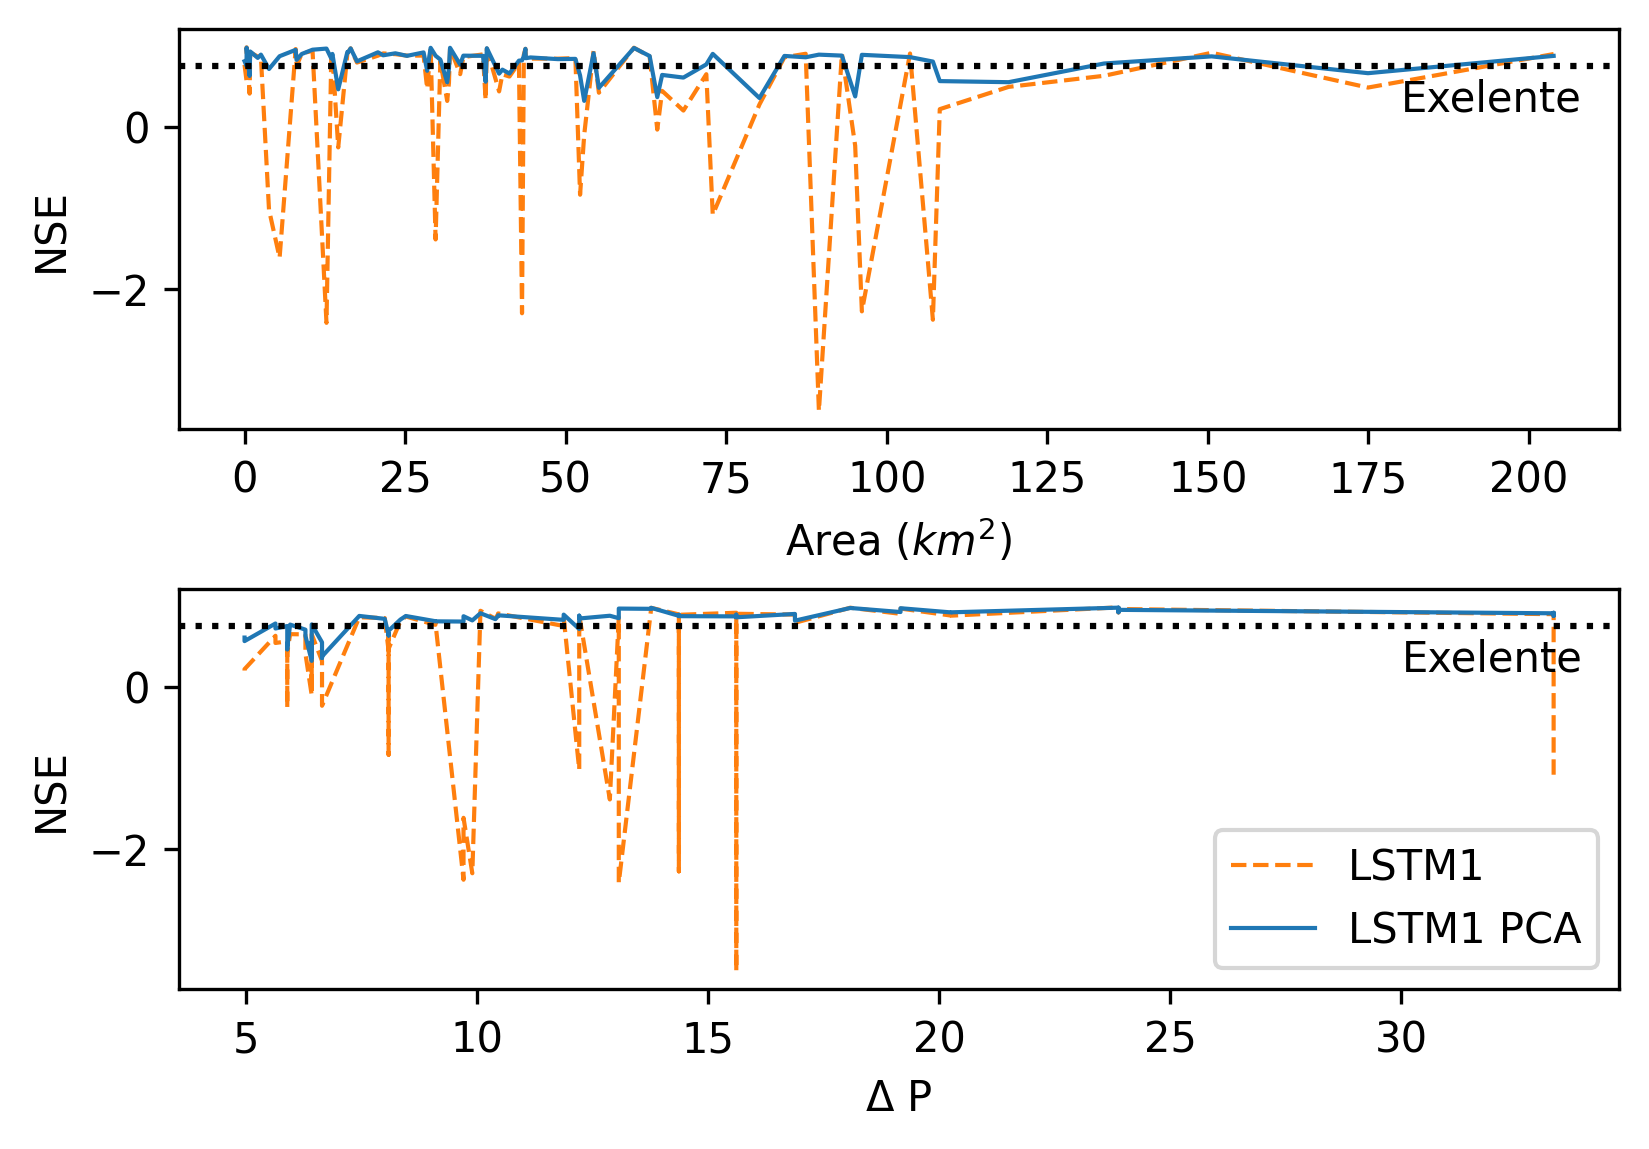
\includegraphics[height=3.5in]{Figures/NSE/comp_NSE_consinPCA.png}
      \caption{ Evolución del coeficiente NSE en función del área (panel superior) y la variación de precipitación 
      (panel inferior) para los modelos LSTM1 con y sin PCAs.}
      \label{NSEs_Area_prec}
    \end{center}
  \end{figure}


En la figura \ref{NSEs_Area_prec}, se muestra la comparación entre los valores de NSE obtenidos para el modelo LSTM1 con PCAs 
(curva continua) y sin PCAs (curva a rayas) en función del área de la cuenca (panel superior) y de la variación de precipitación 
(panel inferior). Los resultados obtenidos cuando consideramos las 288 características
de entrada muestran una gran fluctuación de los valores de NSE y en general peores predicciones. 
Una razón por la que las componentes principales funcionan mejor puede deberse a que éstas agregan la información proveniente de 
todo el dominio del espacio predictor \cite{Manu}. En línea con este argumento, en estas figuras también se puede observar que el 
área de las sub-cuencas y la variación de precipitación son factores relevantes que condicionan la calidad de los ajustes. 
El modelo que no incluye componentes principales  tiende a fallar más en las cuencas pequeñas ($Area  < 120~km^2$) y 
áridas  ($\Delta P < 20~mm/d$). Esto puede deberse a que en estos casos los 
valores de la precipitación y caudales son más pequeños y el loss es en general menor  que el loss para una sub-cuenca con
una descarga grande. Esto último provoca que el modelo deje de aprender demasiado pronto y se genere un
un sobre peso para las sub-cuencas más grandes y húmedas mientras que la performance en las 
más pequeñas y áridas disminuye \cite{Kratzert}.

\begin{figure}[h!]
  \begin{center}
    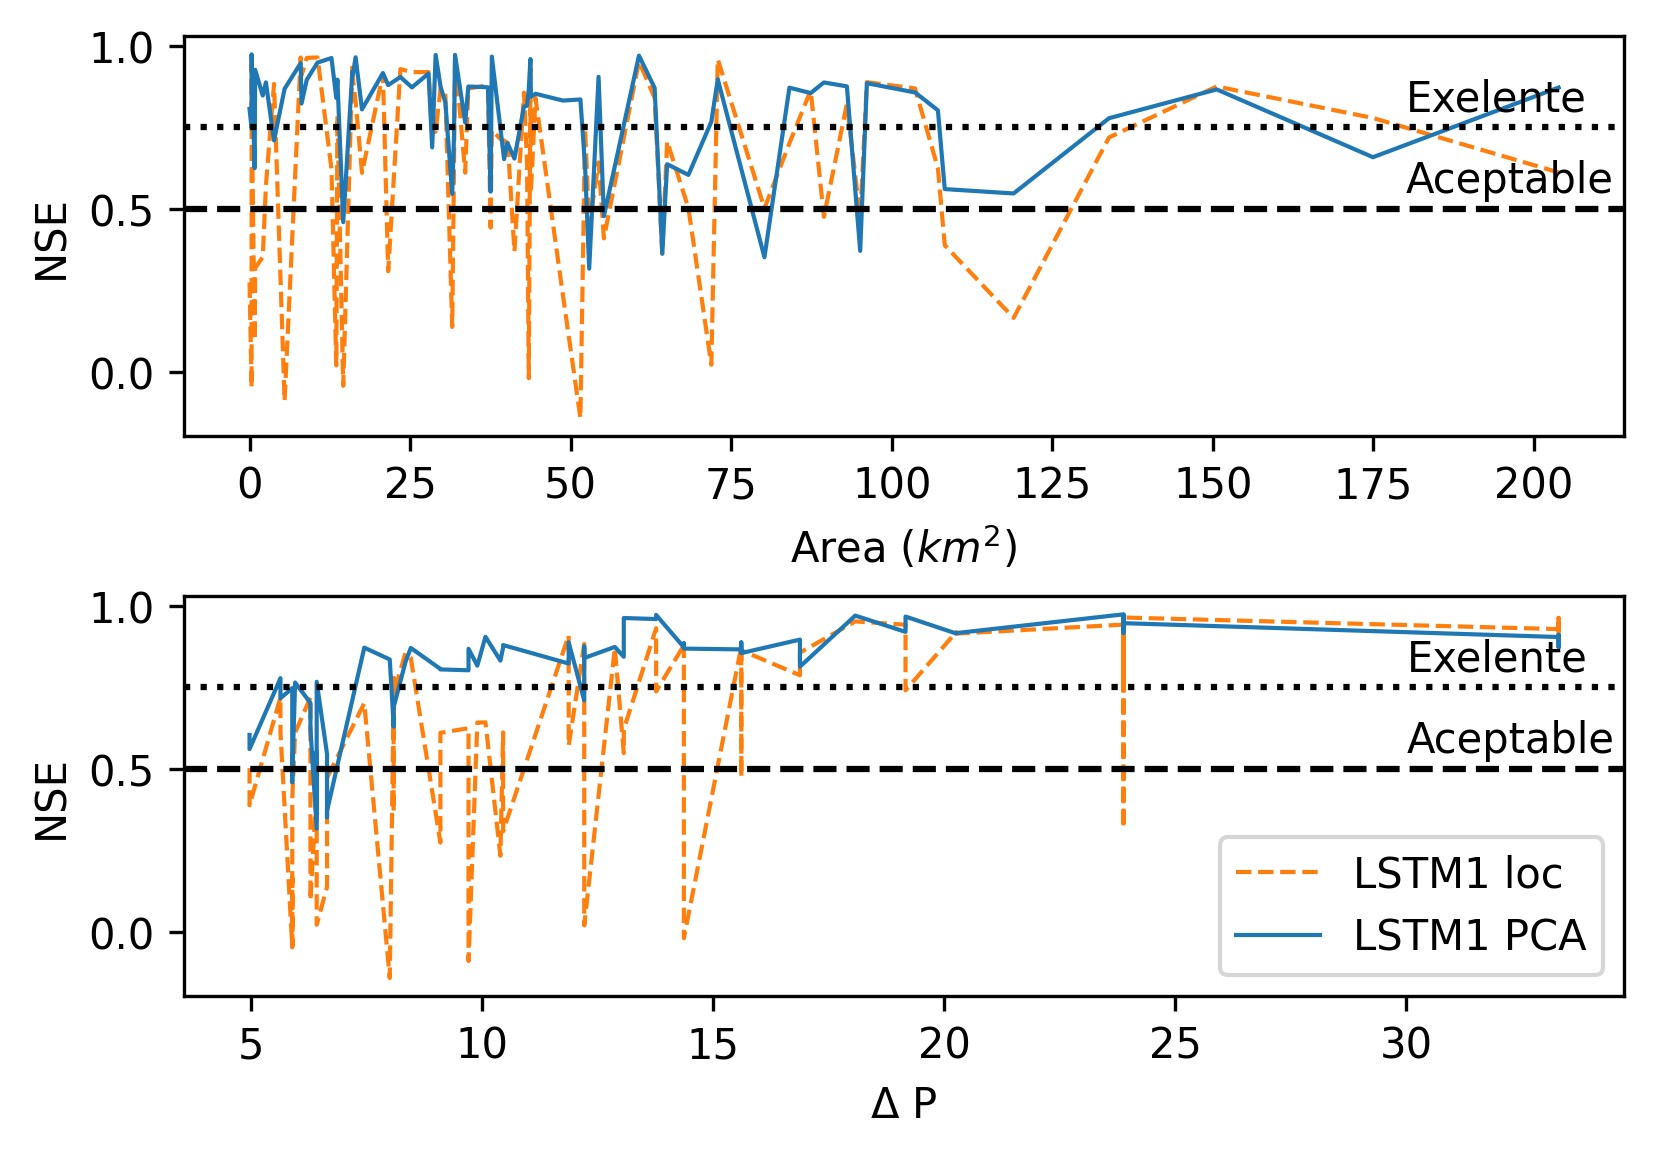
\includegraphics[height=3.5in]{Figures/NSE/comp_NSE_consinPCA2.png}
    \caption{ Evolución del coeficiente NSE en función del área (panel superior) y la variación de precipitación 
    (panel inferior) para los modelos LSTM1 con PCAs y LSTM1 entrenado localmente.}
    \label{NSE3}
  \end{center}
\end{figure}




% the MSE from a basin with low average discharge (e.g., smaller, arid basins) is generally smaller than the MSE from a basin 
% with high average discharge (e.g., larger, humid basins). We need an objective function that does not depend on basin-specific 
% mean discharge so that we do not overweight large humid basins (and thus perform poorly on small, arid basins).

Este efecto es también visible cuando entrenamos el modelo LSTM1 de manera local,
como puede verse en la figura \ref{NSE3} en la mayoría de los casos, la performance del modelo global  es 
mejor que la del modelo local. Este resultado se encuentra alineado con estudios 
que demuestran que los modelos LSTM entrenados en un gran número de sub-cuencas son capaces de vincular Las
características de las mismas para aprender un modelo global que a su vez es capaz de reflejar  
explícitamente las similitudes y diferencias de las cuencas a nivel local  \cite{Kratzert}. 


\begin{figure}[h!]
  \begin{center}
    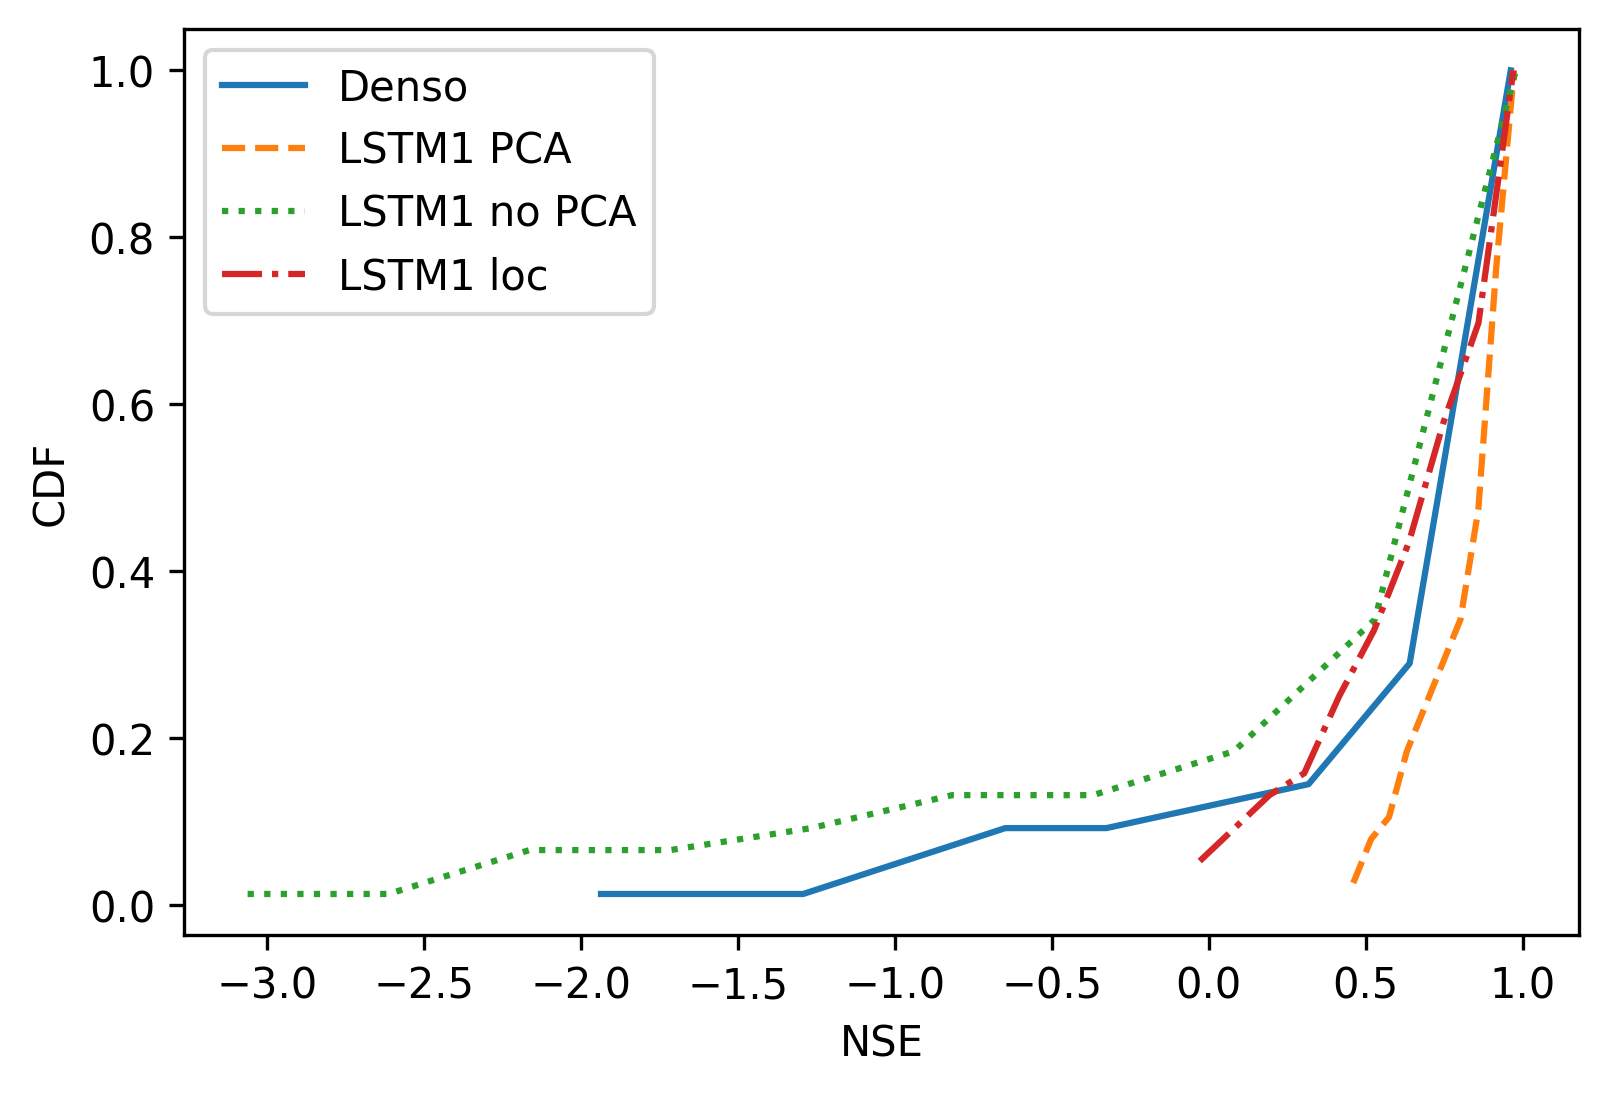
\includegraphics[height=3.5in]{Figures/NSE/CDF.png}
    \caption{ Función de distribución acumulada para todos los modelos de ANNs a lo largo de todas las sub-cuencas de CHRC.}
    \label{CDF}
  \end{center}
\end{figure}

En la figura \ref{CDF}, se muestra una comparación de la función de distribución acumulada para todos los modelos sobre las 76 sub-cuencas de CHRC.
En esta figura se puede ver claramente que el modelo que mejor funciona en general es el LSTM1 PCA. El modelo denso es el segundo mejor en algunos
sectores y el que muestra la peor performance en toda la cuenca es el modelo que usa el espacio predictor sin hacer el análisis de componentes principales.

\section{Predicción de los caudales naturales}


\begin{figure}[h!]
  \begin{center}
    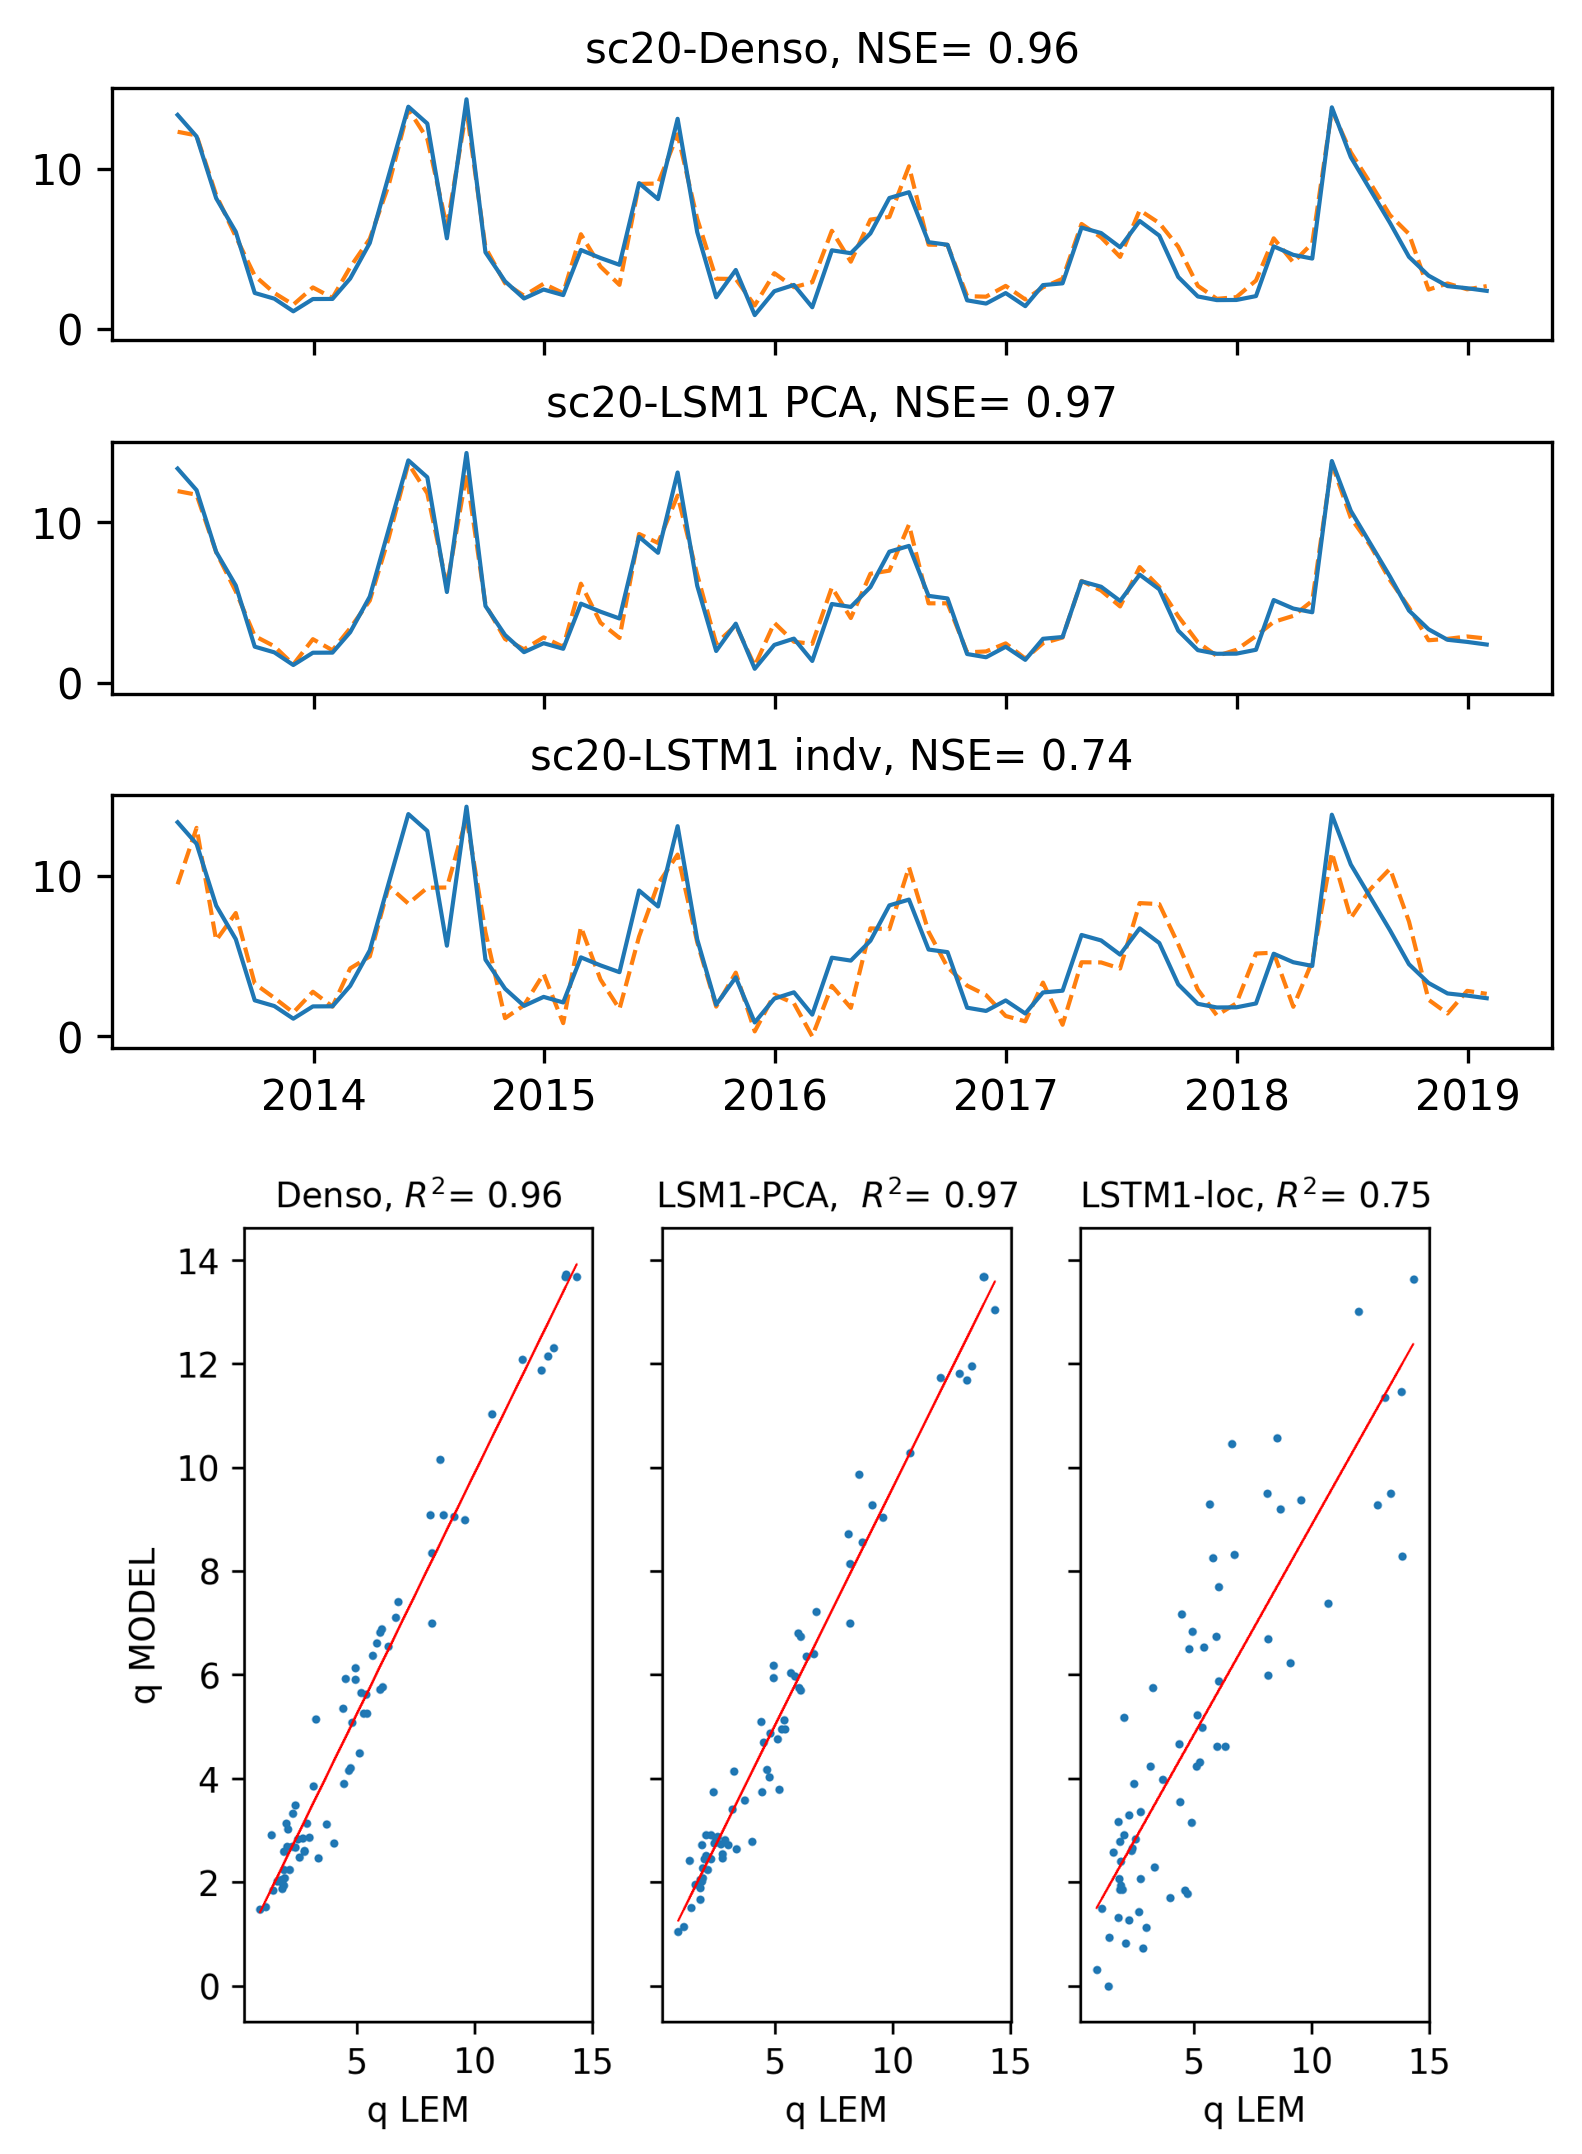
\includegraphics[height=6.in]{Figures/comp_grilla/resultados_sc20}
    \caption{ Predicciones del caudal de descarga obtenidos con los modelos Denso, LSTM1 con PCAs y LSTM1 local en la subcuenca 
    con id 20. En los
    paneles inferiores se muestran los grados de ajuste correspondientes.}
    \label{alcomp20}
  \end{center}
\end{figure}



En las figuras \ref{alcomp20} se muestran  los resultados obtenidos para los caudales en la sub-cuenca con id 20
y los grados de ajustes correspondientes obtenidos con los diferentes modelos.
Las curvas continuas son los valores simulados con el modelo MELCA y las curvas a rayas son los valores predichos 
con los modelos denso, LSTM1 PCA y LSTM1 loc en el conjunto de test. En este caso la performance de los modelos
LSTM1 PCA y denso es excelente, con valores de NSE iguales a 0.97 y 0.96, respectivamente, 
mientras que el modelo entrenado localmente es un poco más baja. Como se ha explicado en sesiones anteriores, los
modelos entrenados de manera global con componentes principales, aprenden en un espacio que contiene información agregada
proveniente de todo el espacio predictor. El ajuste del modelo LSTM1 PCA es aún mejor porque la presencia de neuronas recurrentes 
permiten contemplar la correlación de los datos en la dimensión temporal.




\begin{figure}[h!]
  \begin{center}
    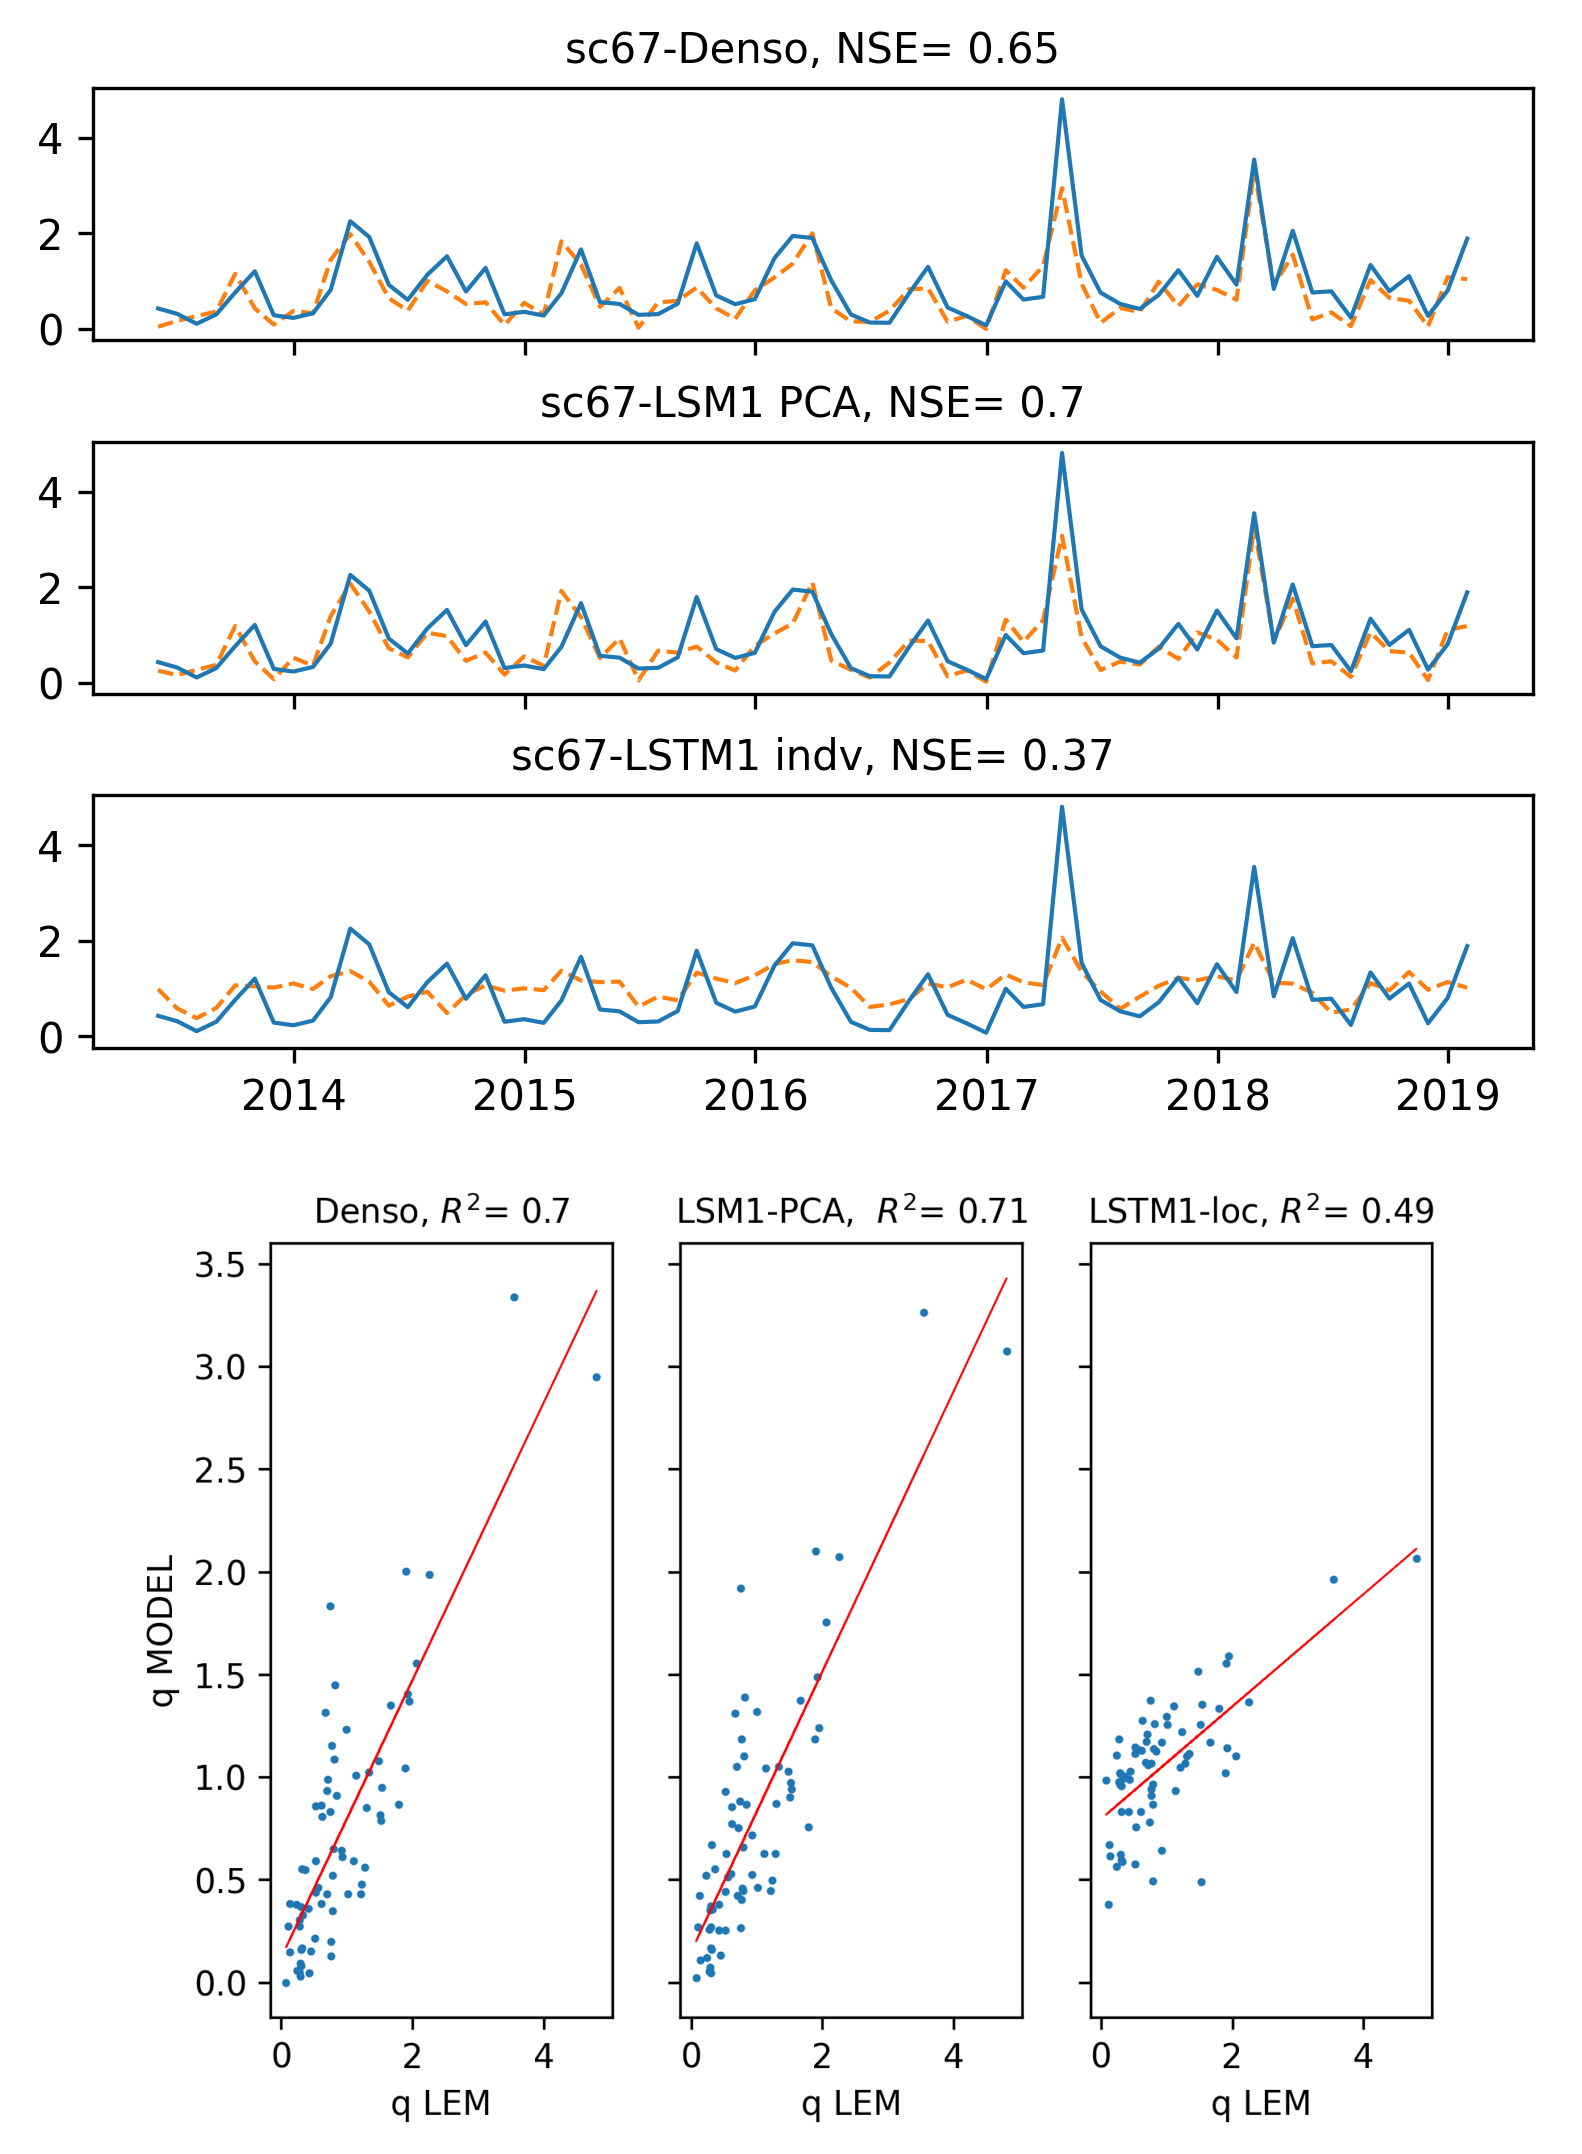
\includegraphics[height=6.in]{Figures/comp_grilla/resultados_sc67.png}
    \caption{ Predicciones del caudal de descarga obtenidos con los modelos Denso, 
    LSTM1 con PCAs y LSTM1 local en la subcuenca con id 67. En los
    paneles inferiores se muestran los grados de ajuste correspondientes.}
    \label{alcomp67}
  \end{center}
\end{figure}

En la figura \ref{alcomp67} se muestra  a modo de ejemplo un caso en el que el modelo LSTM1 loc falla 
al predecir los valores en el conjunto de test, mientras que los modelos Denso y LSTM1 PCA arrojan un ajuste aceptable
 ($NSE>0.6$). En este caso, el modelo LSTM1 loc ha sido capaz de reflejar 
cierta tendencia de los datos pero aún así la calidad del ajuste es baja ($NSE<0.5$). El modelo LSTM1 PCA, que 
posee ambas ventajas, la de considerar componentes principales y redes recurrentes, es capaz de predecir los valores de los caudales
en el conjunto de test con una calidad buena ($NSE=0.7$). 

 
\begin{figure}[h!]
\begin{center}
  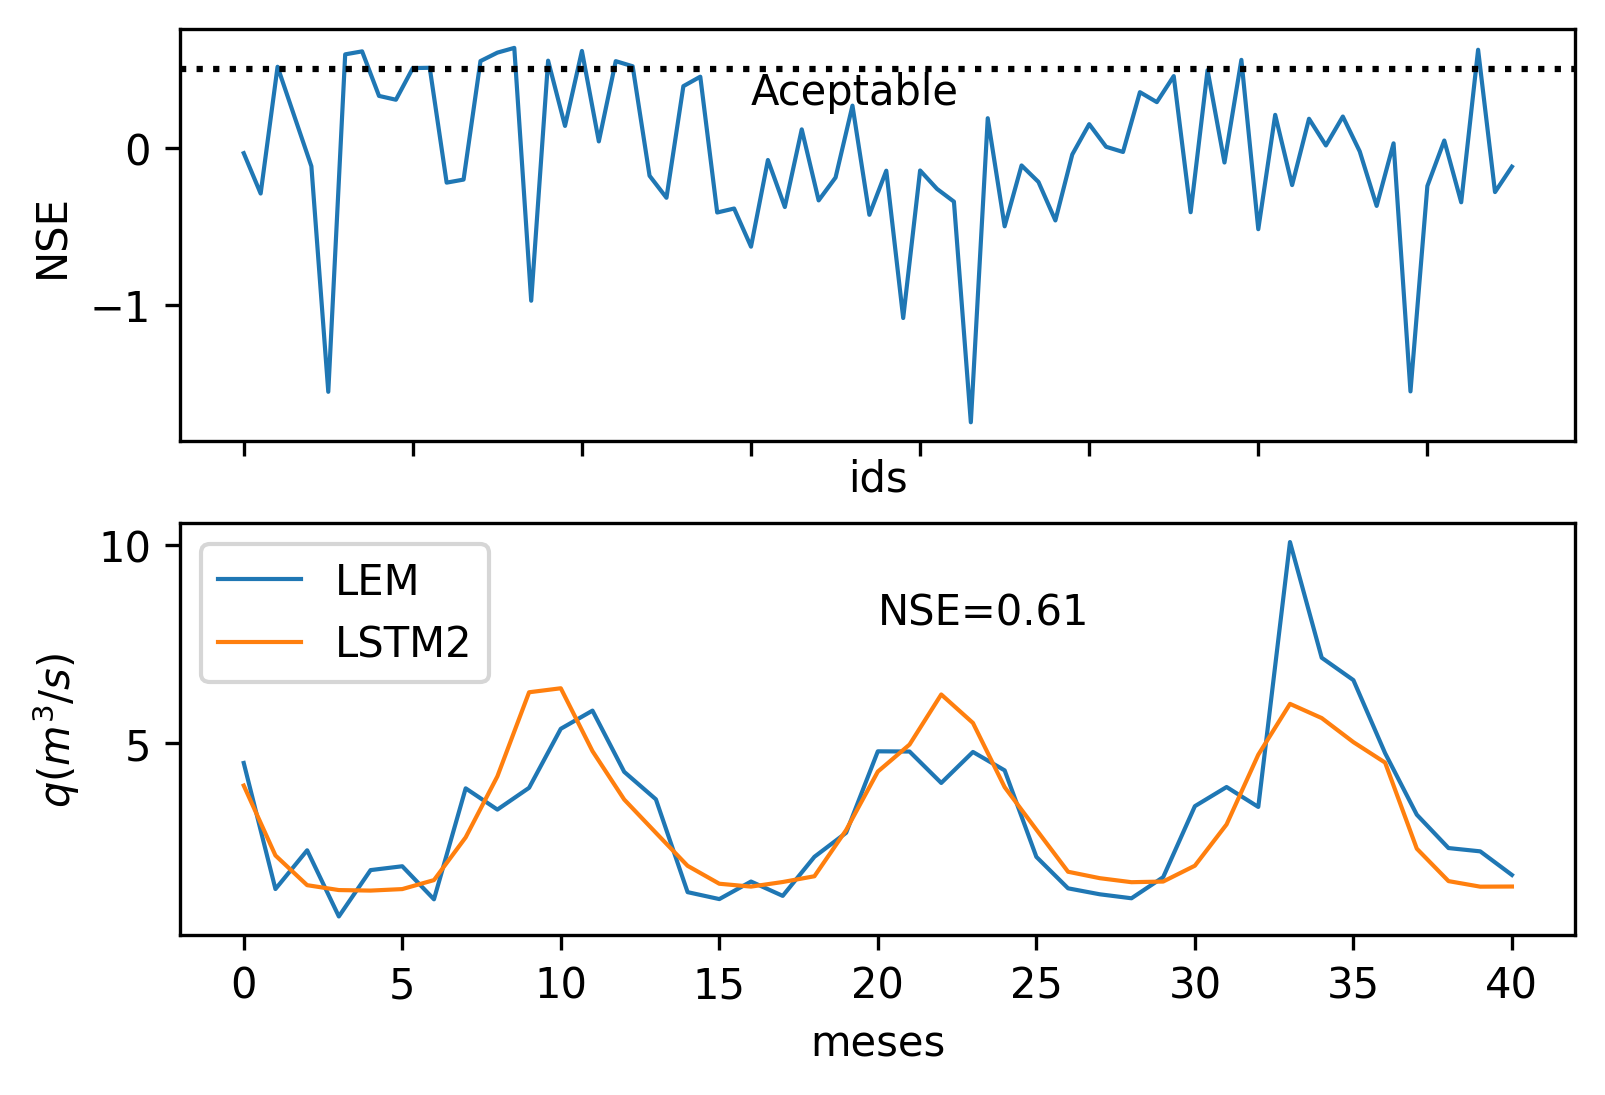
\includegraphics[height=2.8in]{Figures/seq/results_seq.png}

  \caption{ Resultados del Modelo LSTM2. En el panel superior se muestran los valores de NSE a lo largo de toda la cuenca y En
  el panel inferior, los valores predichos en la sub-cuenca con id 15. }
  \label{seq15}
\end{center}
\end{figure}

En la figura \ref{seq15} se muestran los resultados obtenidos para el modelo LSTM2 entrenado secuencialmente. 
en el panel superior se muestran lo valores del coeficiente NSE a lo largo de toda la cuenca
y en el panel inferior los resultados obtenidos para el mejor ajuste. Se puede observar que
la performance del modelo es en general bastante pobre, sólo unos pocos puntos sobrepasan en umbral de calidad aceptable.
Los mayores problemas que presenta esta aproximación es que por un lado los errores cometidos en cada una de las
predicciones es propagado y acumulado a lo largo del tiempo y por otro lado se pierde completamente
la información otorgada por las series hidro-climáticas de entrada, por lo cual el modelo no es capaz de aprender ningún 
patrón relacionado con la respuesta que las diferentes sub-cuencas tienen frente a las series de precipitación.  






%   \begin{center}
%     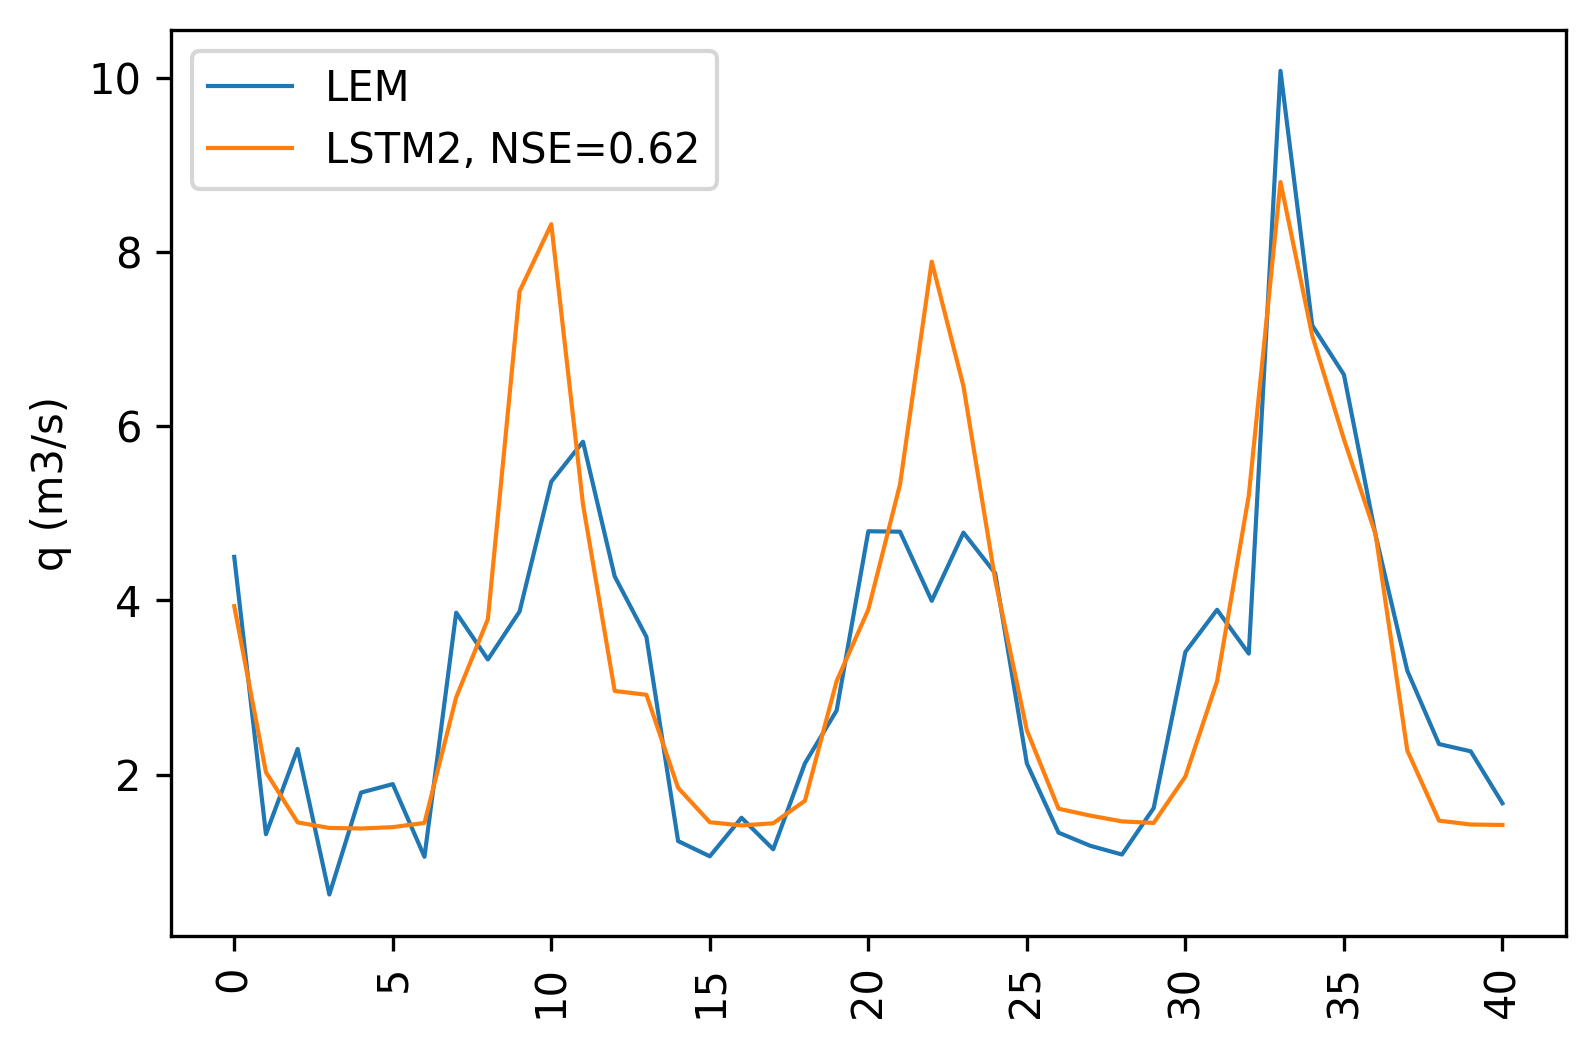
\includegraphics[height=2.5in]{Figures/seq/seq_sc15.png}
%     \caption{ Resultados del Modelo LSTM 2.}
%     \label{seq15}
%   \end{center}
% \end{figure}


% #* Graficas de las distribuciones de los pesos? para ver que patrones se forman?

% \begin{figure}[h!]
%     \begin{center}
%       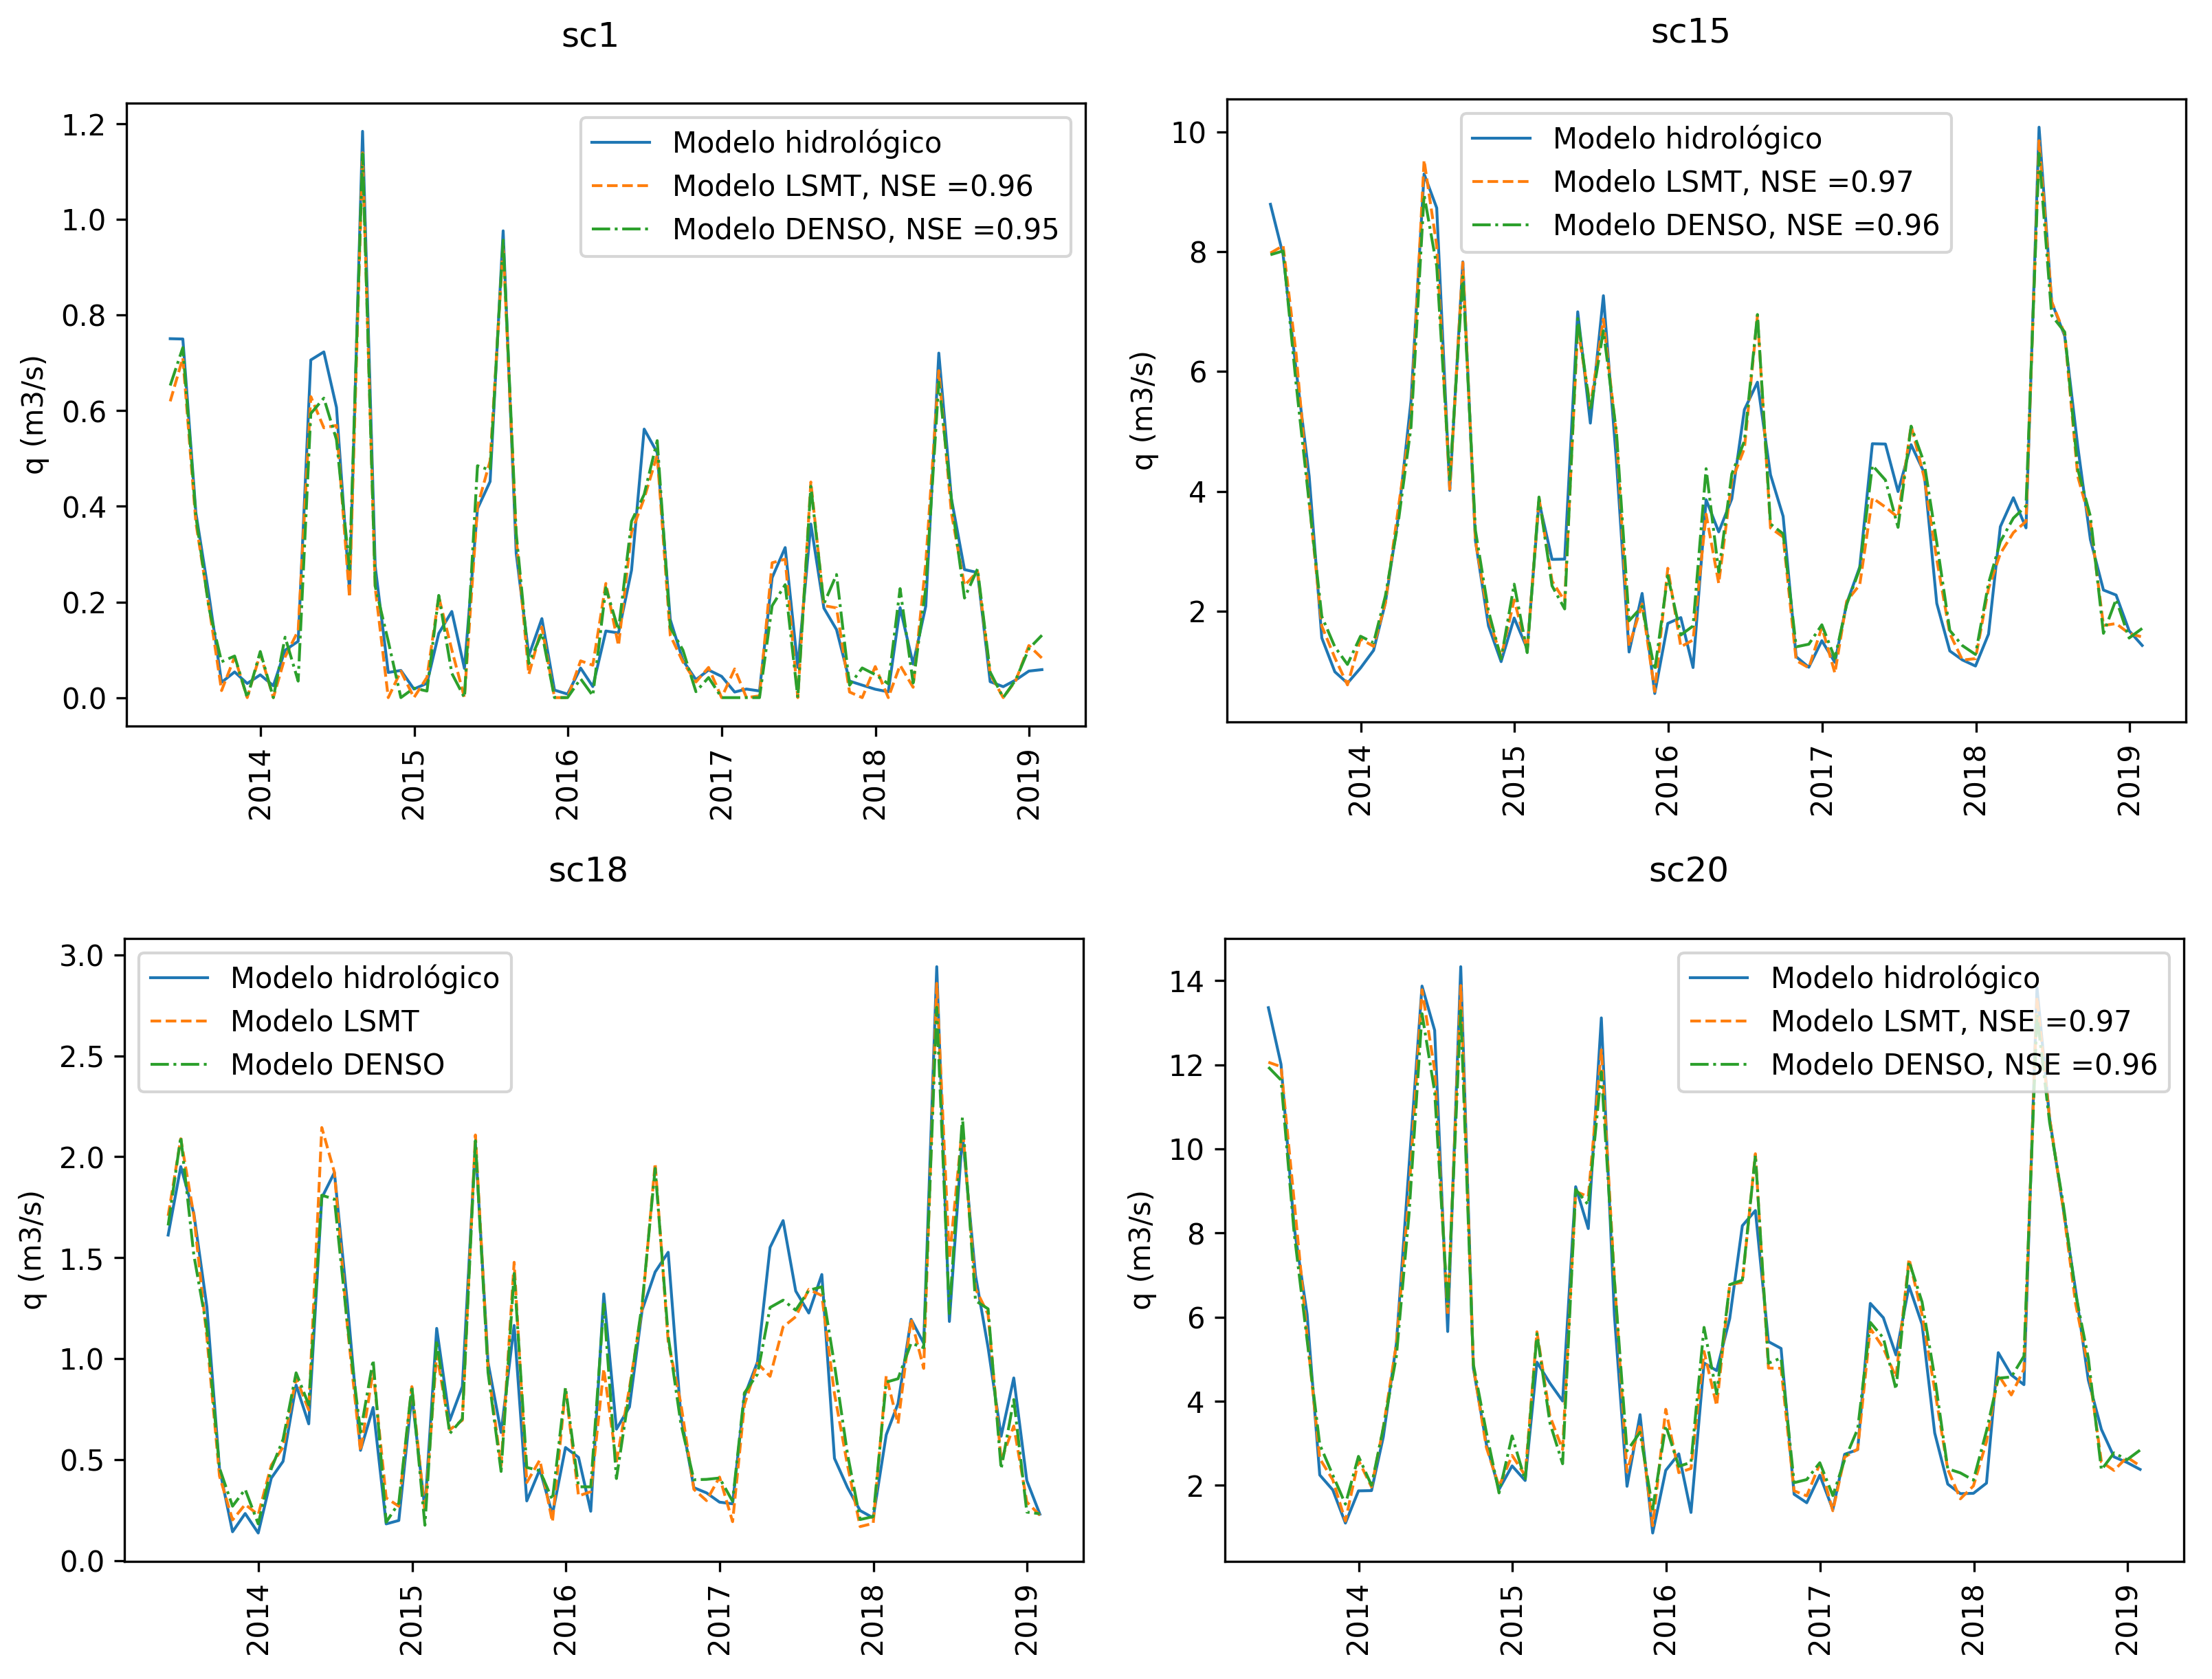
\includegraphics[height=4.in]{Figures/comparacion_scs.png}
%       \caption{ Resultados del Modelo LSTM 2.}
%       \label{autocorrelacion}
%     \end{center}
%   \end{figure}





% \begin{figure}[h!]
%     \begin{center}
%       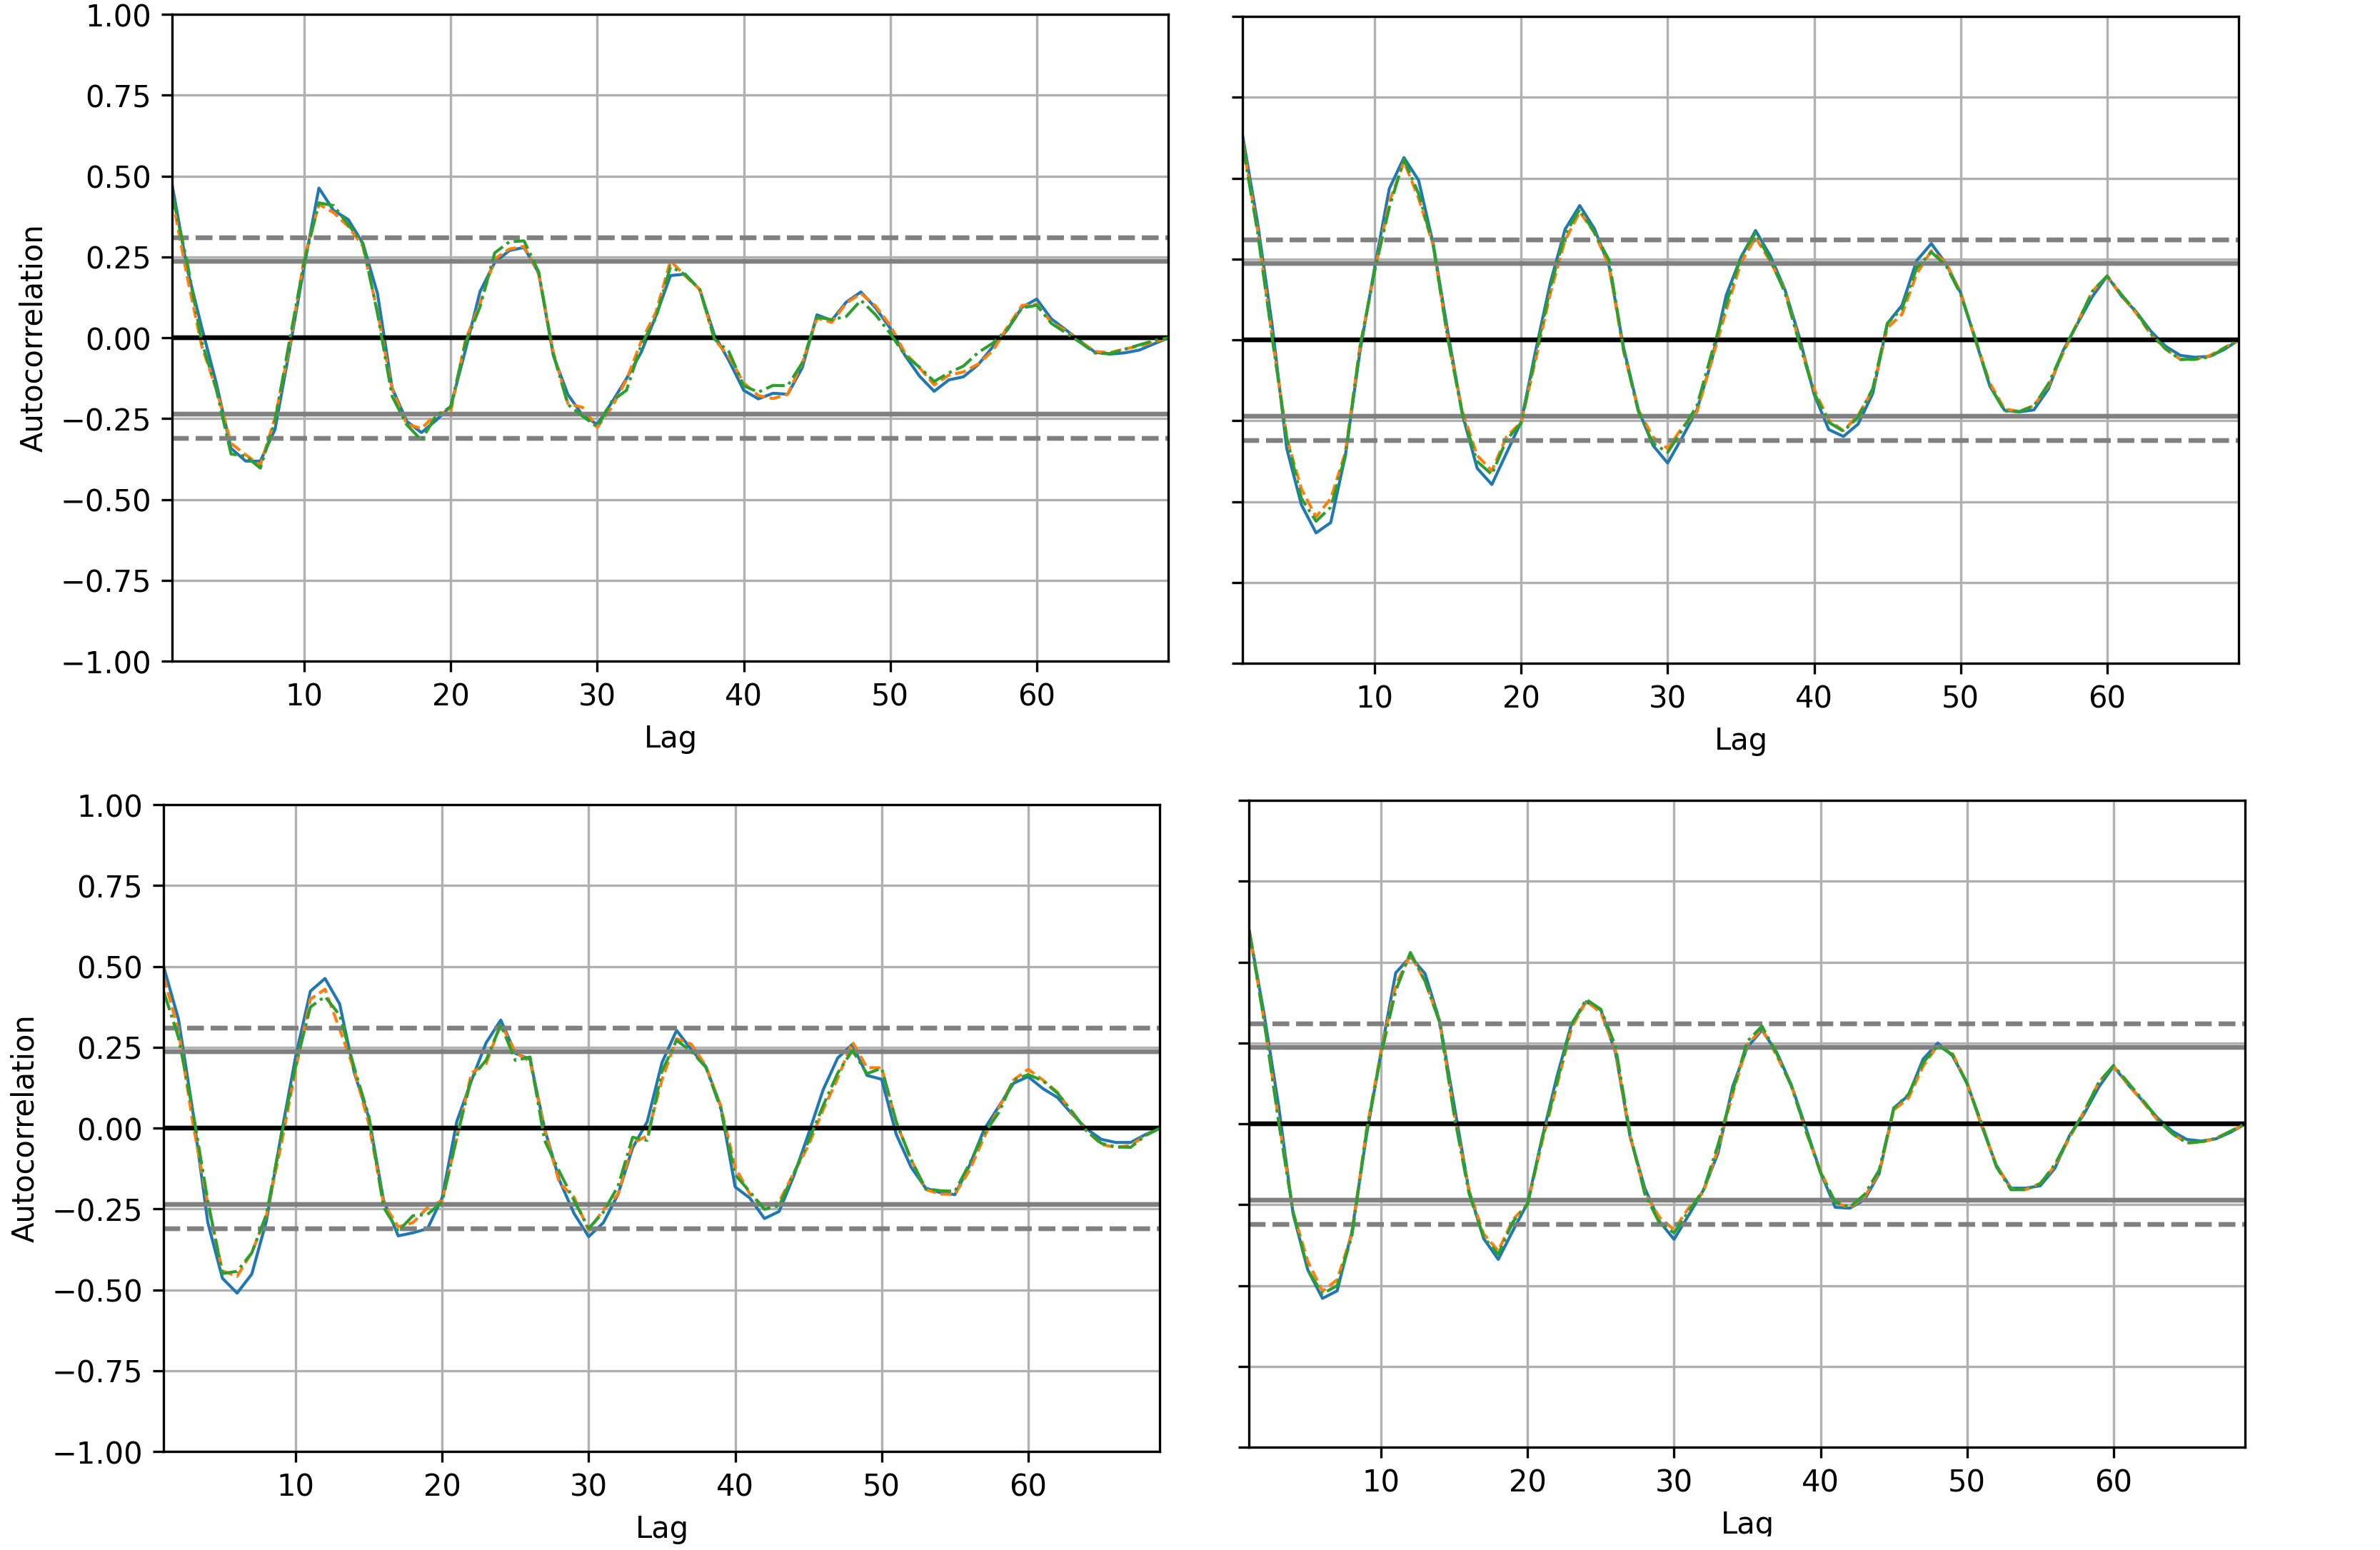
\includegraphics[height=3.5in]{Figures/autocorr_scs.png}
%       \caption{ Funciones de autocorrelación.}
%       \label{resultados_q}
%     \end{center}
%   \end{figure}

% En la figura \ref{autocorrelacion} se muestran las funciones de autocorrelación
% correspondientes a cada una de la subcuencas. Se puede observar que ambos modelos son capaces de captar correctamente 
% la estacionalidad de los datos.



%  \begin{figure}[h!]
%     \begin{center}
%       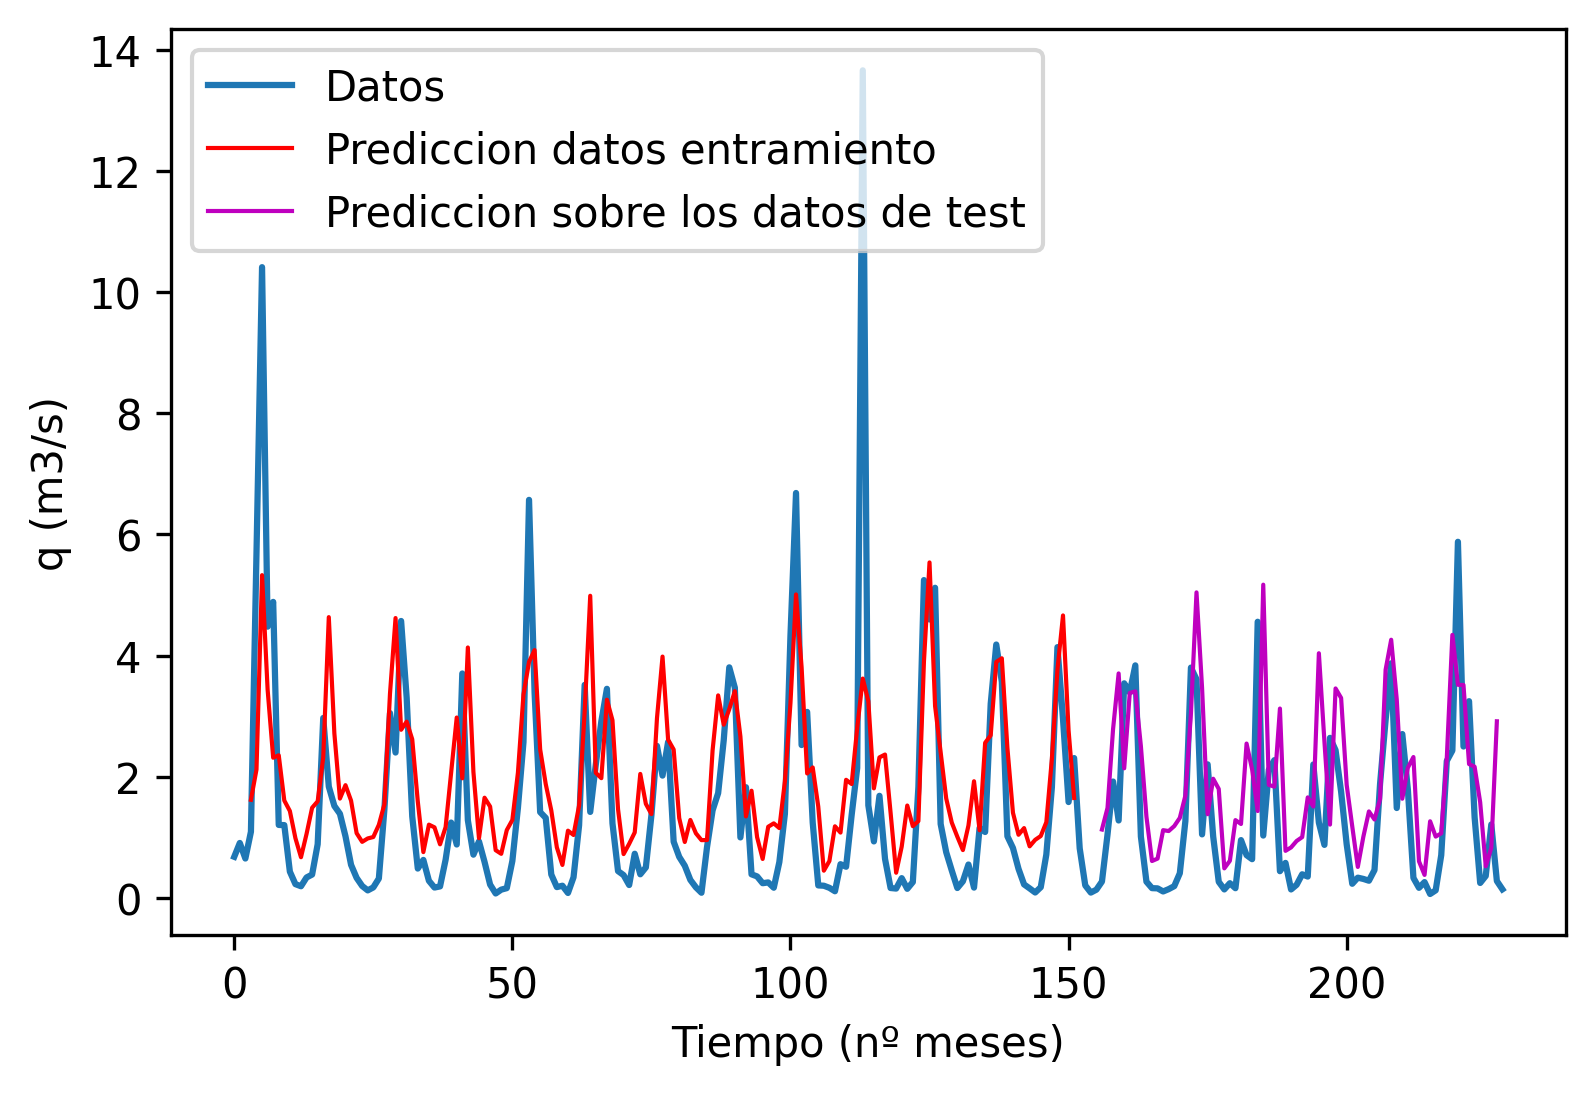
\includegraphics[height=3.in]{Figures/modelo_LSTM_seq.png}
%       \caption{ Resultados del modelo LSTM 3.}
%       \label{result_LSTM3}
%     \end{center}
%   \end{figure}


%   En la figura \ref{result_LSTM3} se muestran los resultados obtenidos con el modelo LSTM3 en todo el rango de datos 
%   para la subcuenca numero 73. En este enfoque, se han predicho los datos de manera secuencial, 
%   para lo cual sólo se ha utilizado la información de las series temporales de los caudales simulados en el
%   conjunto de entrenamiento. Si bien este modelo predice   correctamente la tendencia de los datos, 
%   falla al predecir los valores de los caudales.

  





% %   \begin{figure}[h!]
% %     \begin{center}
% %       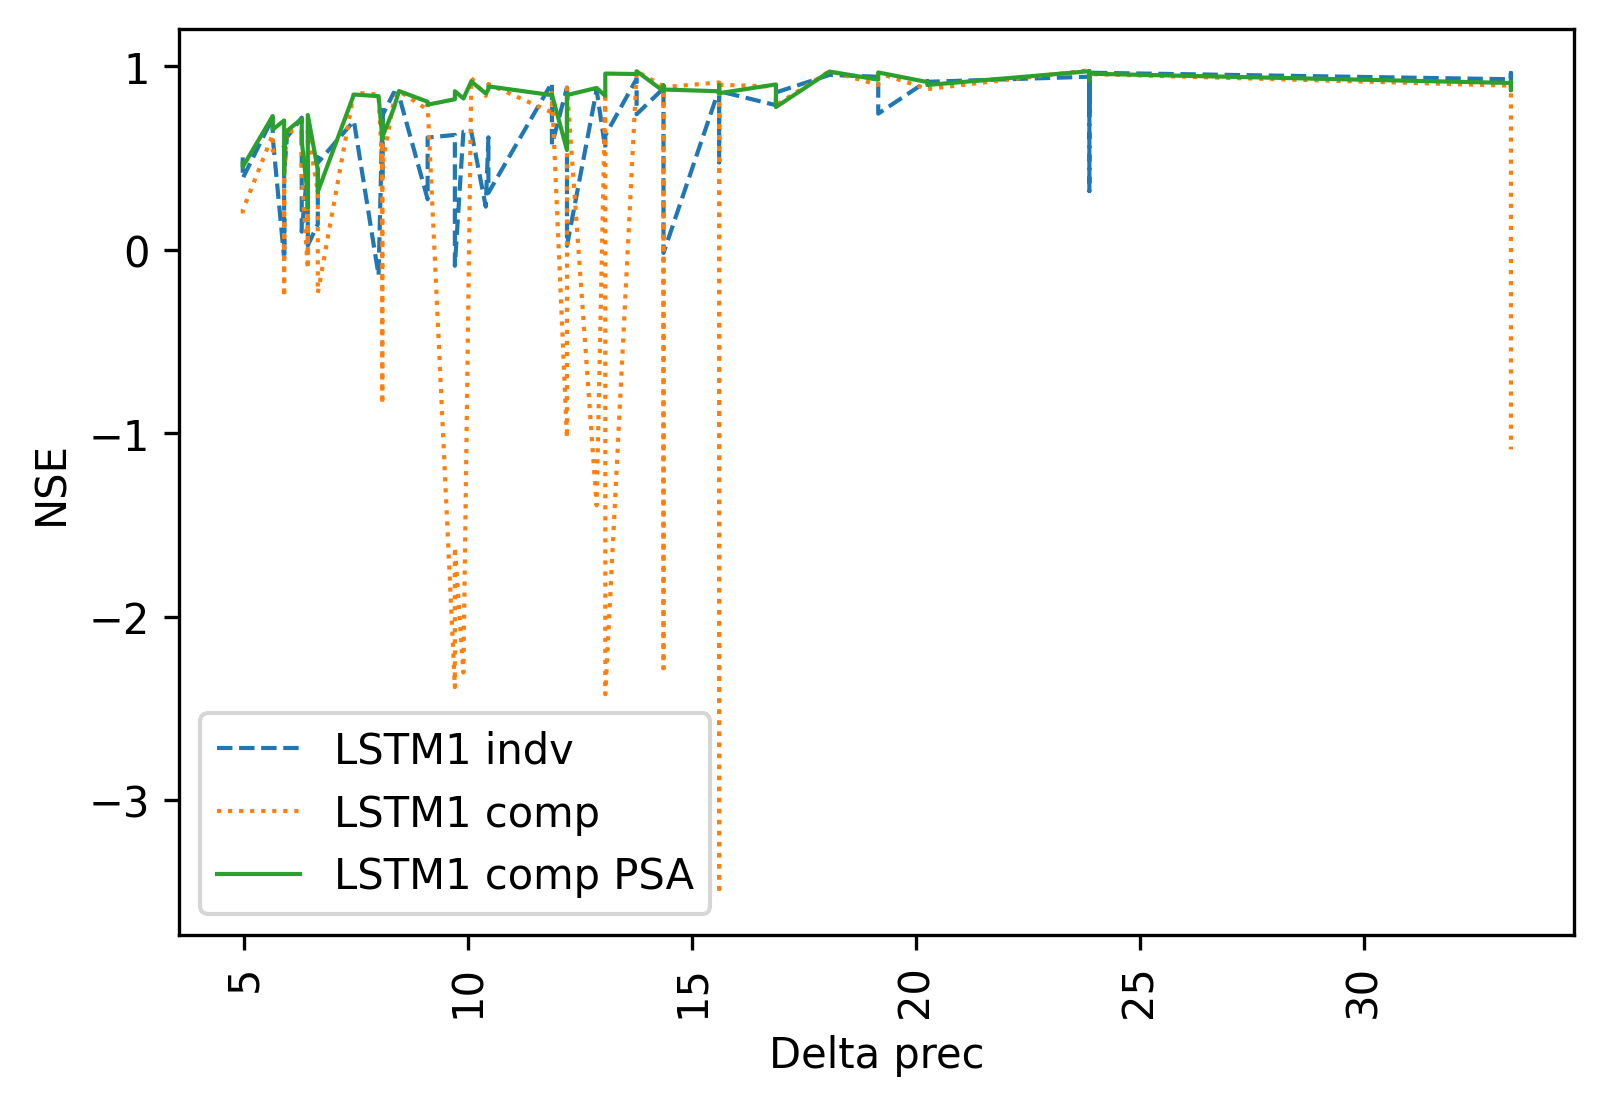
\includegraphics[height=2.in]{Figures/NSEs_Delta prec.png}
% %       \caption{ Modelo LSTM 2}
% %       \label{Red_LSTM2}
% %     \end{center}
% %   \end{figure}

\section{Cálculo de balance hídrico con MODSIM}


Con el fin de determinar si los resultados obtenidos con redes neuronales pueden ser utilizados para simular 
operaciones en la cuenca CHRC, se ha determinado el balance hidrológico utilizando el software MODSIM (introducido en \ref{Modelo_balance})
con los caudales simulados por el modelo hidrológico MELCA y las predicciones de los modelos
de redes neuronales en el conjunto de test.

En el panel superior de la figura \ref{modsim}  se muestra el residuo ($R$), es decir la diferencia entre los valores de los 
caudales predichos respecto a los caudales de referencia (en este caso simulados con el modelo MELCA), 
para diferentes sub-cuencas distribuidas a lo largo de toda la cuenca hidrográfica Chambo. 
En los paneles inferiores se muestran los valores de los caudales  arrojados por MODSIM  para la sub-cuenca que se encuentra
a la salida de CHRC (aguas abajo) y para una de las sub-cuencas que se encuentra a mayor altitud (aguas arriba). 
Las curvas continuas corresponden al resultado obtenido con los caudales simulados con el modelo MELCA, 
y la curva a rayas es el resultado obtenido cuando consideramos los valores predichos por el modelo LSTM1 PCA. 
Se puede apreciar que los resultados arrojados por MODSIM son los mismos para ambos casos, es decir, 
las pequeñas variaciones mostradas en el panel superior no influyen en el resultado final. 



  \begin{figure}[h!]
    \begin{center}
      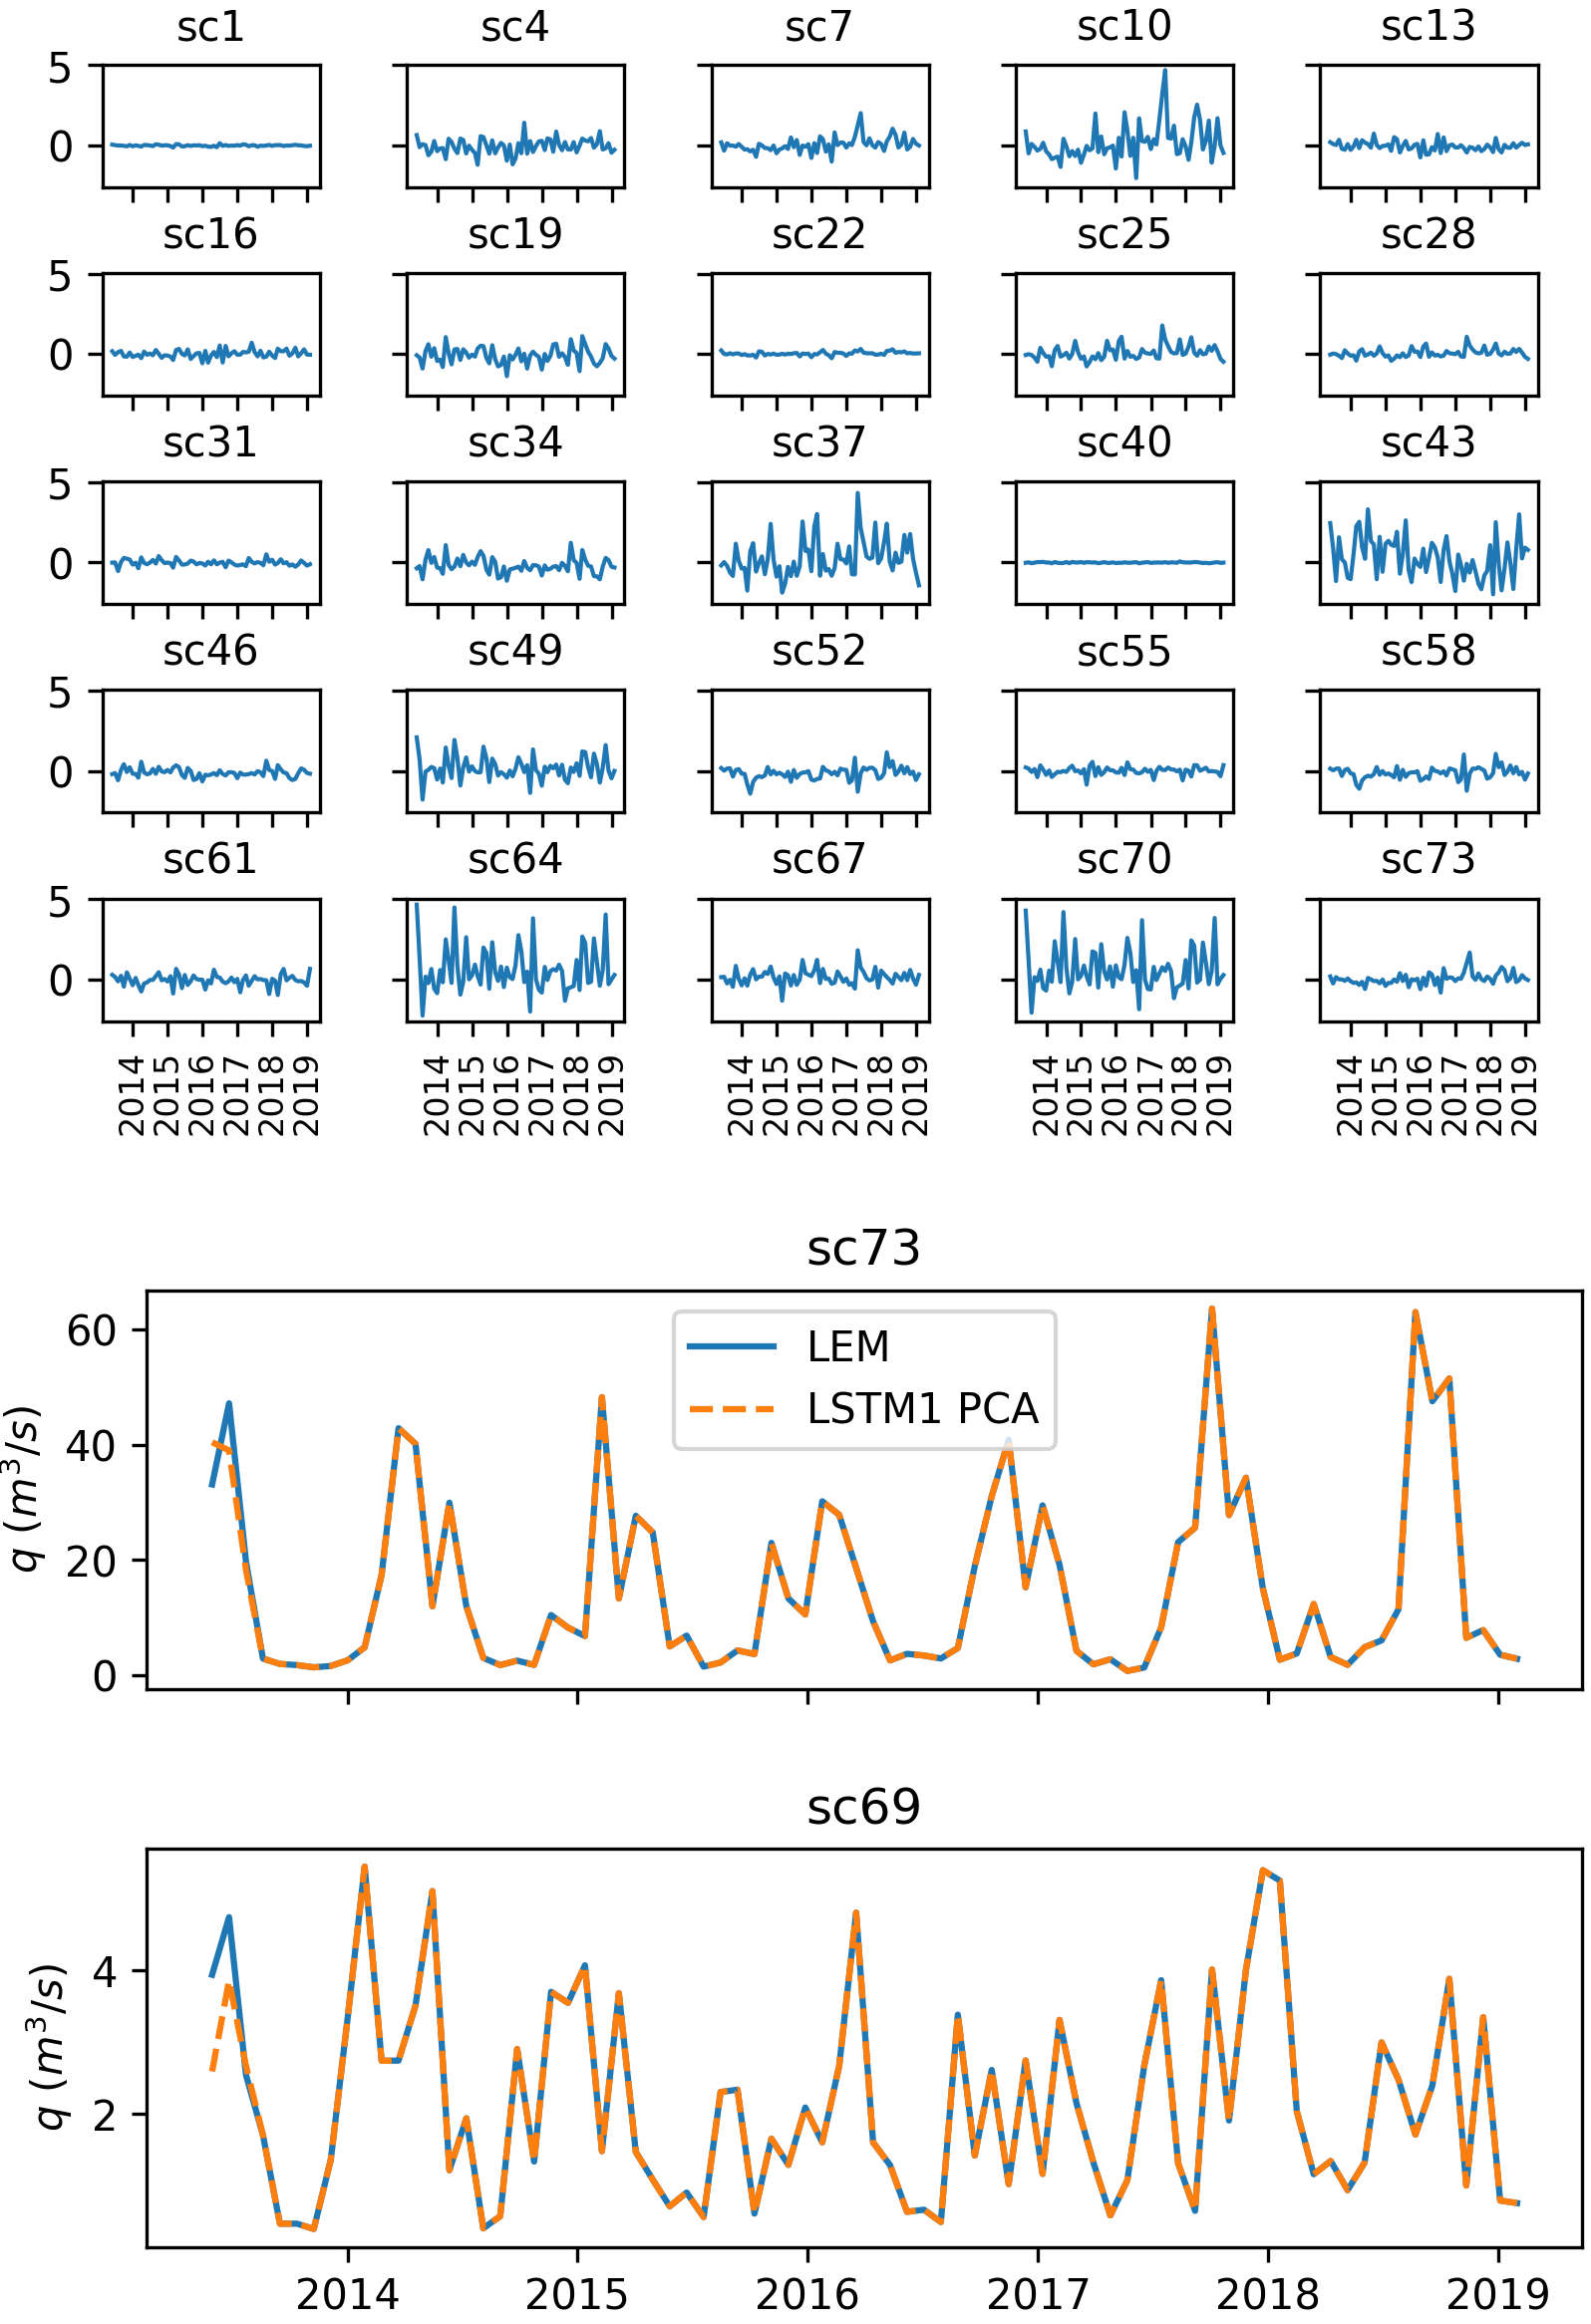
\includegraphics[height=6.5in]{Figures/modzim/comp_modzim.png}
      \caption{ Paneles superiores: residuos obtenidos a lo largo de diferentes sub-cuencas. 
      Paneles inferiores: resultados finales obtenidos utilizando el software de gestión de recursos MODSIM, teniendo en cuenta los usos del agua.}
      \label{modsim}
    \end{center}
  \end{figure}


  % \begin{figure}
%     \centering
%     \begin{subfigure}[b]{0.6\textwidth}
%         \centering
%         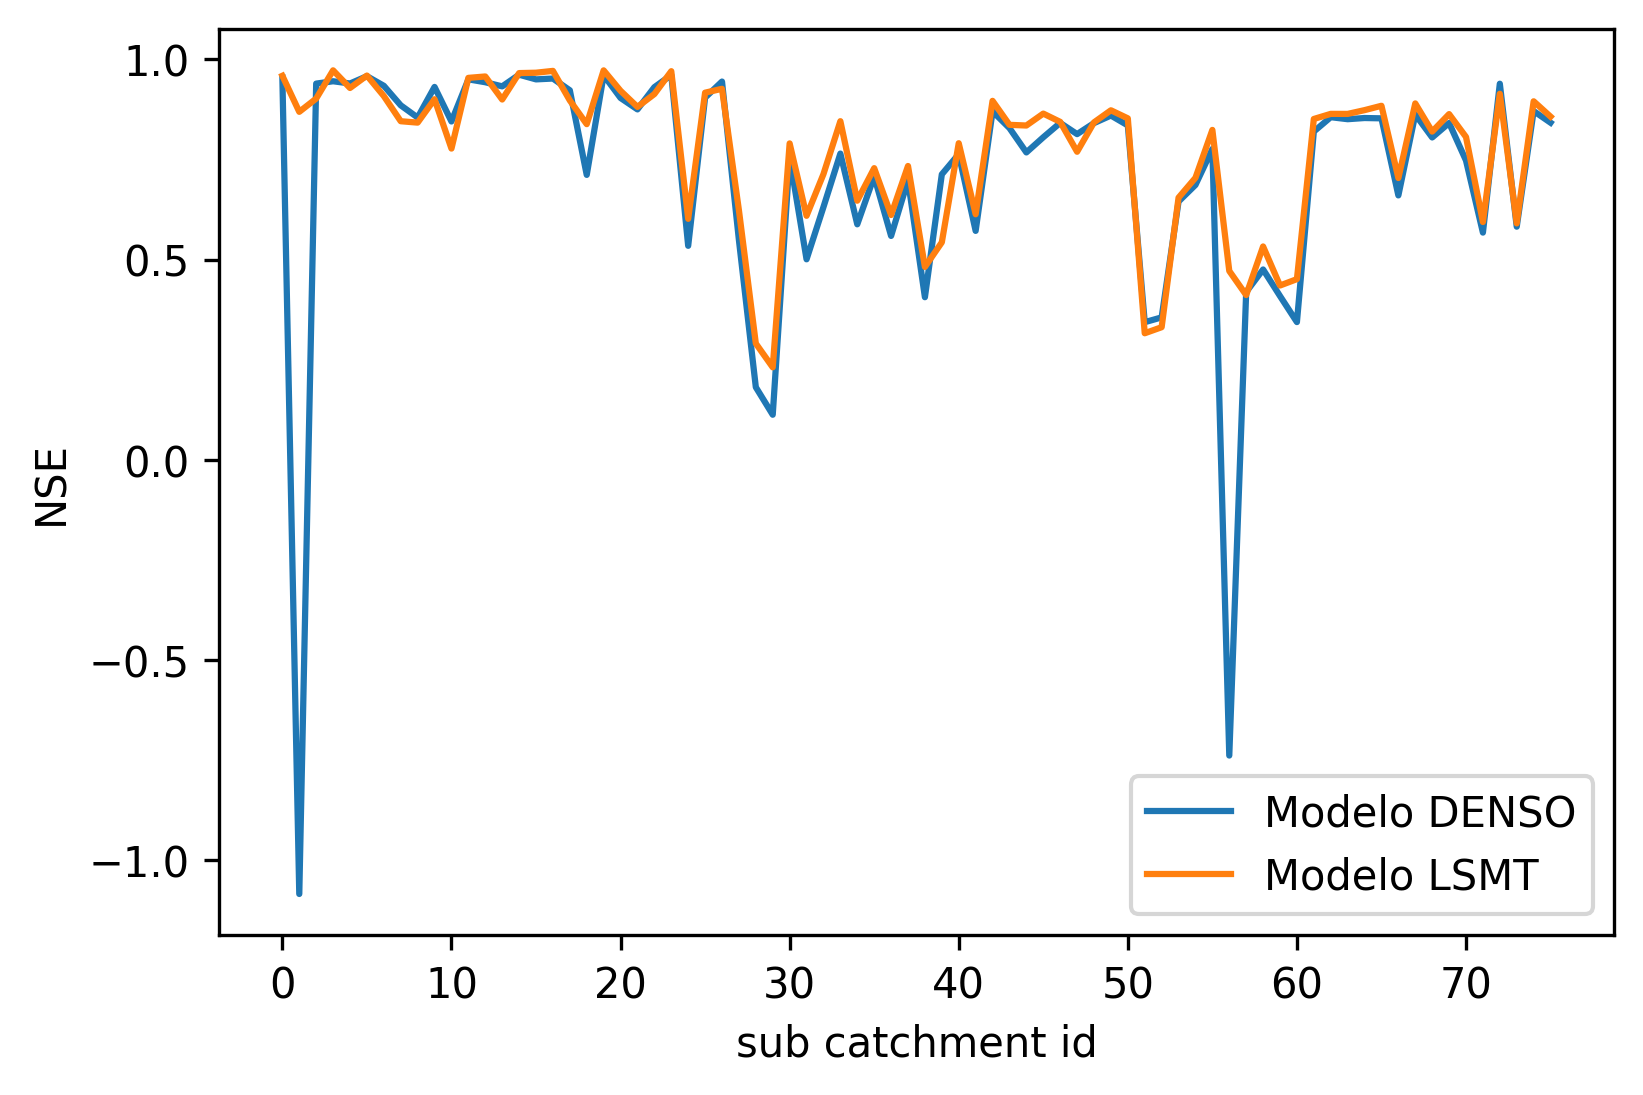
\includegraphics[width=\textwidth]{Figures/comparacion_denso_LSTM_NSE.png}
%         \caption{}
%         \label{fig:y equals x}
%     \end{subfigure}
%     \hfill
%     \begin{subfigure}[b]{0.6\textwidth}
%         \centering
%         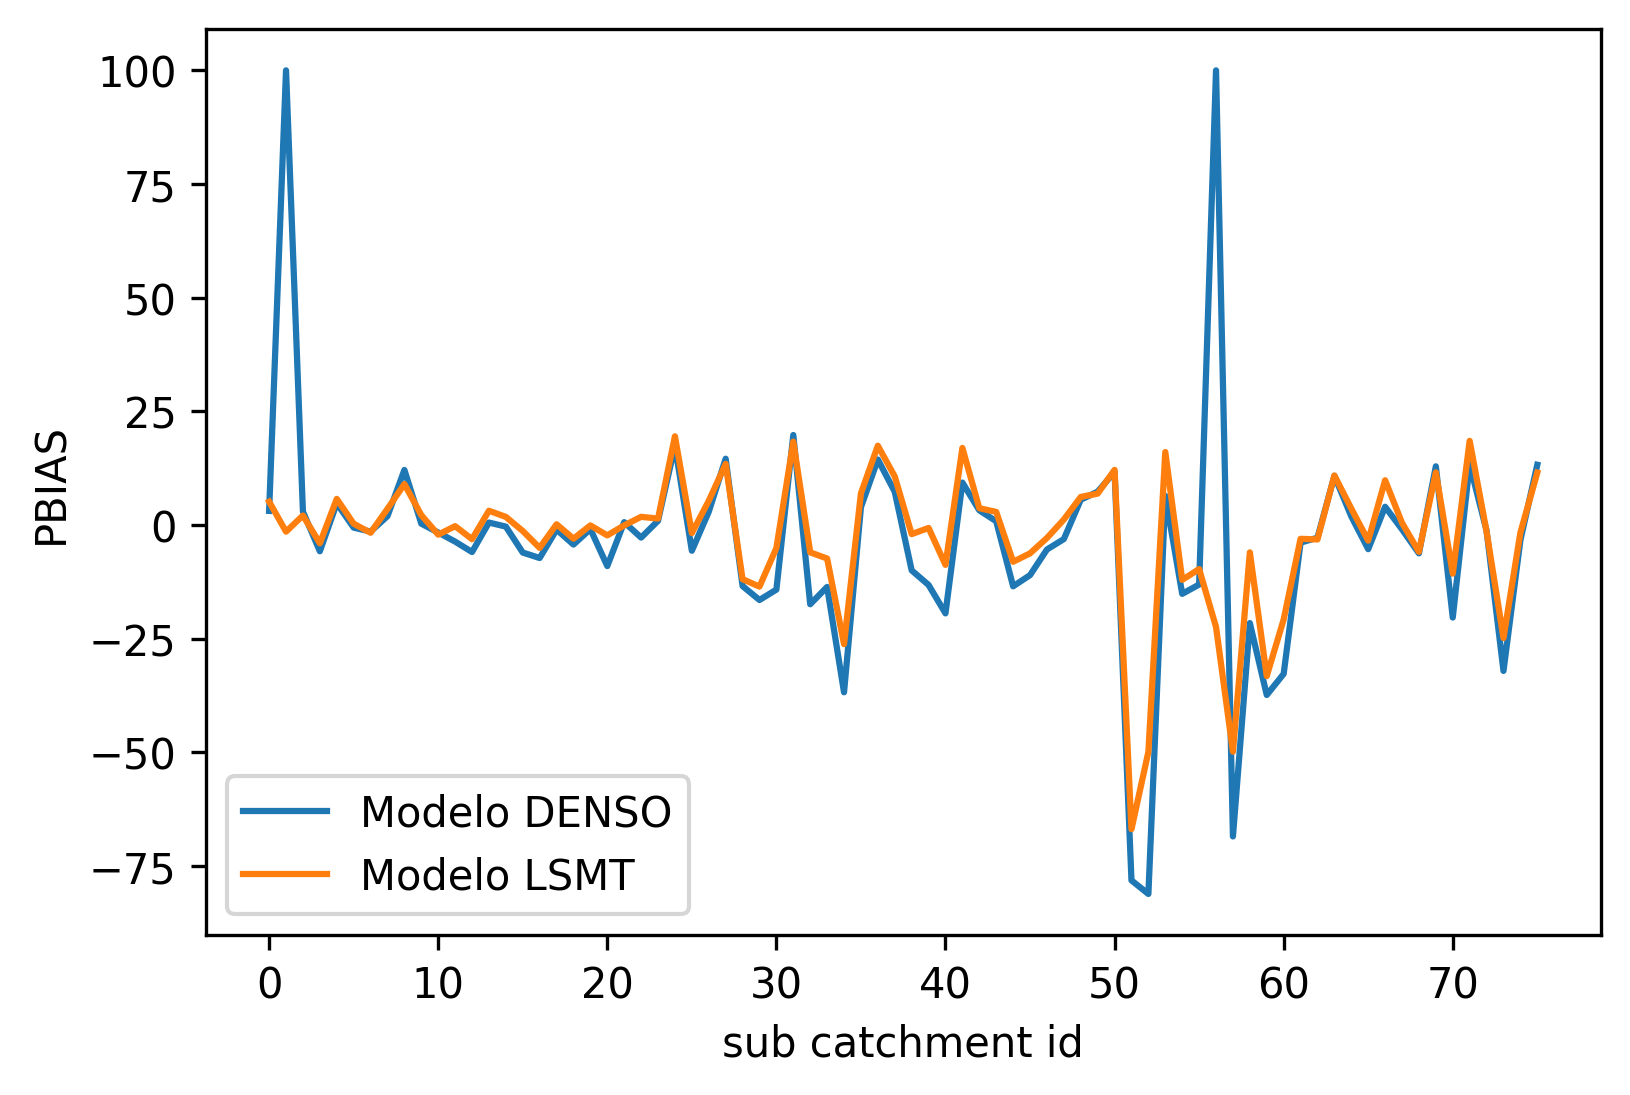
\includegraphics[width=\textwidth]{Figures/comparacion_denso_LSTM_PBIAS.png}
%         \caption{}
%         \label{fig:three sin x}
%     \end{subfigure}
%        \caption{Three simple graphs}
%        \label{fig:three graphs}
% \end{figure}
